\documentclass{beamer}

\usepackage[utf8]{inputenc}
\usepackage{booktabs}
\usepackage{xcolor}
%\usetheme{Hannover}
\usecolortheme{crane}
\usepackage{siunitx,cancel}
\usepackage{graphicx}
\usepackage{hyperref}

\usepackage{listings}
\usepackage{color}
\usepackage{xcolor}

%\usepackage[
%backend=biber,
%style=numeric,
%citestyle=numeric,
%sorting=none
%]{biblatex}
%\addbibresource{resources.bib}


% This is the color used for MATLAB comments below
\definecolor{MyDarkGreen}{rgb}{0.0,0.4,0.0}
\definecolor{Blue}{rgb}{0.0,0.0,1.0}
\definecolor{Purple}{rgb}{1.0,0.0,1.0}

\colorlet{mygray}{black!30}
\colorlet{mygreen}{green!60!blue}
\colorlet{mymauve}{red!60!blue}

\lstset{
  backgroundcolor=\color{gray!10},
  basicstyle=\ttfamily,
  columns=fullflexible,
  breakatwhitespace=false,
  breaklines=true,
  captionpos=b,
  commentstyle=\color{mygreen},
  extendedchars=true,
  frame=single,
  keepspaces=true,
  keywordstyle=\color{blue},
  language=c++,
  numbers=none,
  numbersep=5pt,
  numberstyle=\tiny\color{blue},
  rulecolor=\color{mygray},
  showspaces=false,
  showtabs=false,
  stepnumber=5,
  stringstyle=\color{mymauve},
  tabsize=3,
  title=\lstname
}






%\defaultfontfeatures{Scale=MatchLowercase,Mapping=tex-text}
%\setmainfont[Numbers=Lowercase]{Minion Pro}
%\setsansfont[Numbers=Lowercase]{Myriad Pro}
%\setmonofont{Menlo}
%\setmathsfont(Digits,Latin,Greek)[Numbers={Lining,Proportional}]{Minion Pro}

\sisetup{%
  output-decimal-marker = {.},
  per-mode = symbol,
  %round-mode = places,
  %round-precision = 5
}

\DeclareSIUnit \electronvolt {\ensuremath{eV}}
\DeclareSIUnit \lightspeed {\ensuremath{c}}
\DeclareSIUnit \dalton{\ensuremath{u}}
\DeclareSIUnit \echarge{\ensuremath{e}}


\newcommand{\mvec}[2]{
\ensuremath{\left(
\begin{array}{c}
#1\\
#2\\
\end{array}
\right)}
}

\newcommand{\Span}{\ensuremath{\mathrm{Span}}}
\newcommand{\Mat}{\ensuremath{\mathrm{Mat}}}
\newcommand{\R}{\ensuremath{\mathbb{R}}}
\newcommand{\Rno}{\ensuremath{\mathbb{R}\backslash\{0\}}}
\newcommand{\Z}{\ensuremath{\mathbb{Z}}}
\newcommand{\ol}[1]{\ensuremath{\overline{#1} } }
\newcommand{\F}[1]{\ensuremath{\mathbb{F}_{#1} } }

\newif\ifdraft

\drafttrue
%\draftfalse

%Information to be included in the title page:
\title{How physics simulations work: simulating particles in electric and magnetic fields}
%Numerical integration of ordinary differential equations: motion of charged particles in electromagnetic fields}
\author{Nikolaj Roager Christensen}
\institute{Student Colloquium in Physics and Astronomy, Aarhus University}
\date{March 2021}

%\AtBeginSection[]
%{
%ect

%\titlegraphic
%{
%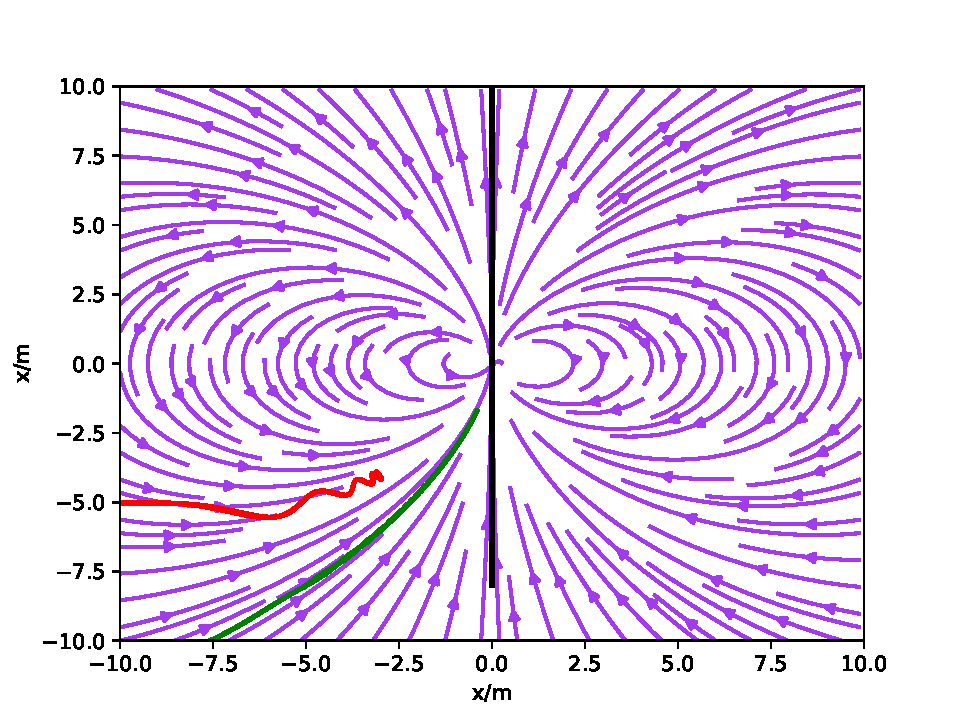
\includegraphics[width=0.5\textwidth]{dipole6.pdf}
%}
\begin{document}

{
\setbeamertemplate{background}
{
    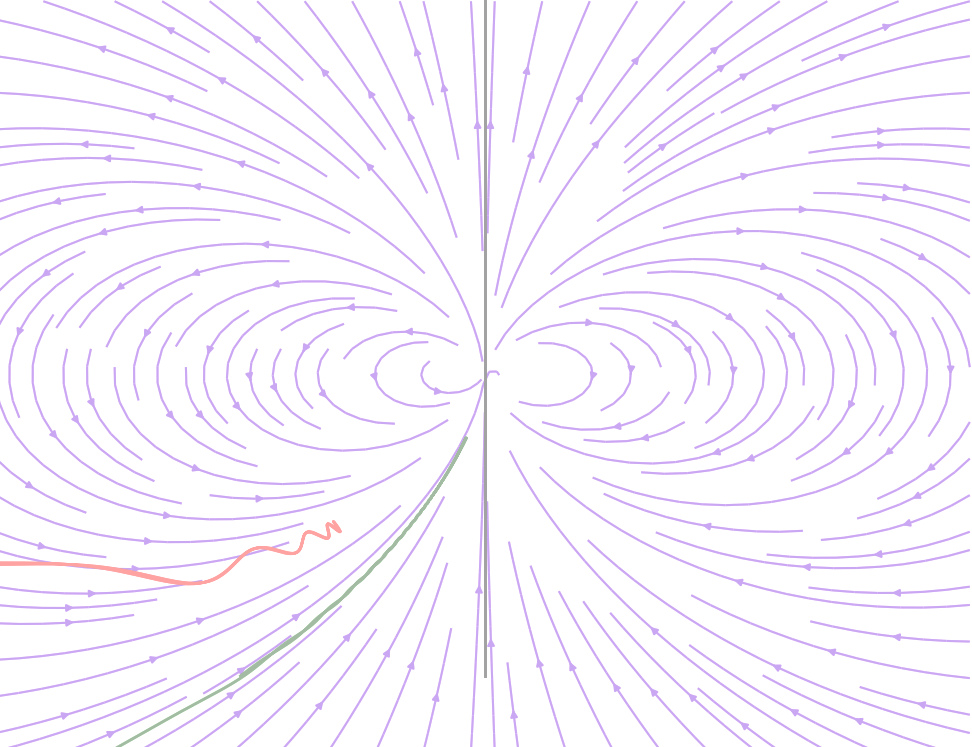
\includegraphics[height=\paperheight]{dipole_preface.png}
}
\frame{\titlepage}
}


\section{Introduction}

\begin{frame}
\frametitle{Numerical integration of ordinary differential equations: motion of charged particles in electromagnetic fields}
\tableofcontents
\end{frame}


\begin{frame}
\frametitle{Introduction, what and why}
\begin{itemize}
\item<1-> Numerical simulations are important.
\item<2-> Testing setups, non-analytical systems.
\item<3-> Demonstration, charged particles in electric and magnetic fields.
\item<3-> Analytically known and not.
\item<4-> Simulations are not experiments!
\end{itemize}
\end{frame}

\ifdraft
    \section{Theory and physical background 10 min}
\else
    \section{Theory and physical background}
\fi

\begin{frame}
\frametitle{Theory: Classical non-relativistic particles}
\begin{itemize}
\item<1-> Some repetition from Electrodynamics
\item<2-> The Lorentz force+N2:

\begin{align*}
\vec{F} &= q ( \vec{v}\times \vec{B}+\vec{E}).\\
m \ddot{\vec{r}}(t) &= q ( \dot{\vec{r}}(t)\times \vec{B}(\vec{r},t)+\vec{E}(\vec{r},t)).
\end{align*}

\item<3-> Only 1 particle! so pre-programmed depending on the setup.

\item<4-> Could use potentials $\phi(\vec{r},t)$ $\vec{A}(\vec{r},t)$ and Hamiltonian, or Lagrangian.

\item<4-> Other systems would have other differential equations.

\end{itemize}
\end{frame}


\begin{frame}
\frametitle{Known results, cyclotron motion $\vec{B}$ fields}
\begin{columns}
\begin{column}{0.5\linewidth}
\begin{itemize}
\item<2-> Magnetic forces do no work:

\begin{equation*}
dW_{\vec{B}}= \vec{F}_B \cdot d\vec{r}\propto (\vec{v}\times \vec{B})\cdot \vec{v} = 0.
\end{equation*}

\item<3-> ($\vec{v}=\vec{v}_\perp+\vec{v}_\parallel$):

\begin{equation*}
|\vec{F}_B| = |q ( \vec{v}\times \vec{B})| =|q v_{\perp} B|.
\end{equation*}
\item<4-> Same as Centripetal force: Cyclotron motion

\item<5-> Cyclotron radius and frequency:

\begin{equation*}
R = \frac{v_\perp m}{|q|B} \quad \omega_c =\frac{|q|B}{m}.
\end{equation*}

\end{itemize}
\end{column}
\begin{column}{0.5\linewidth}
\only<1-2>{%
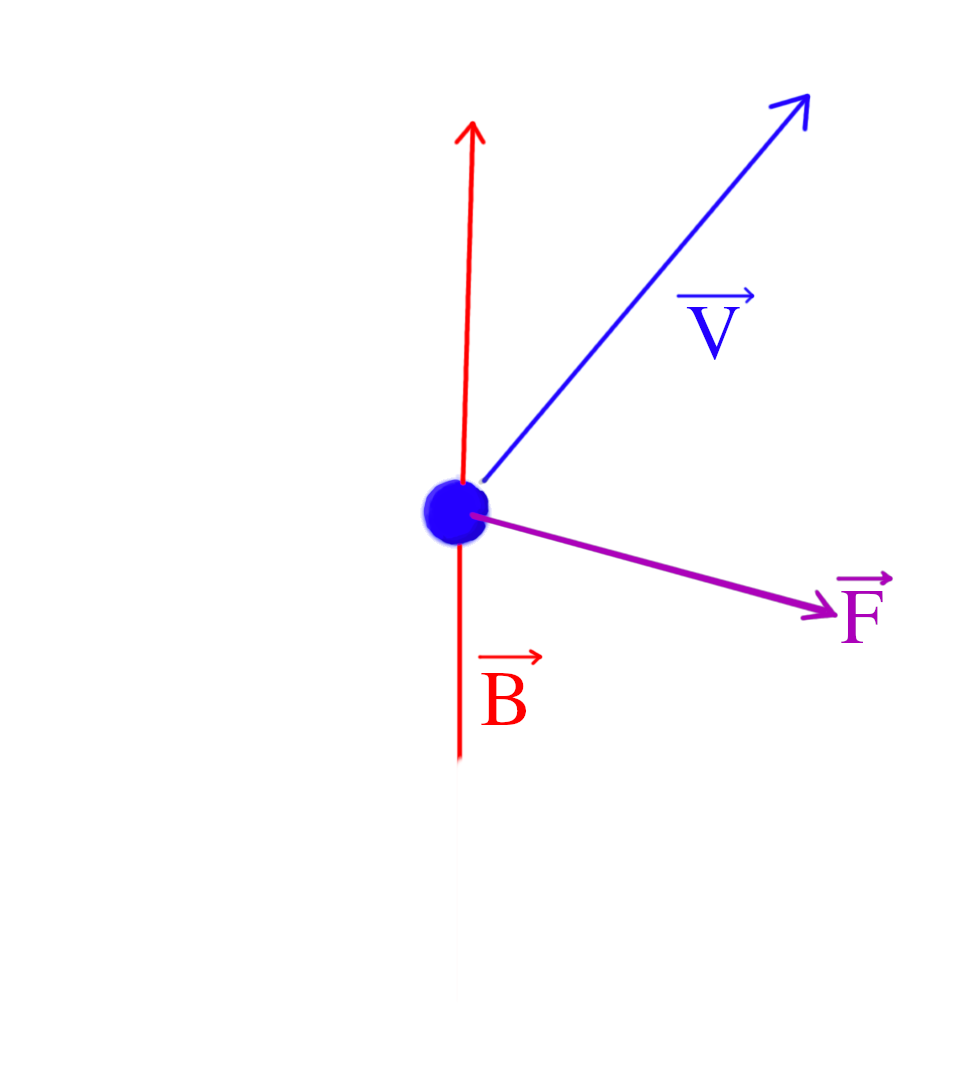
\includegraphics[width=\linewidth]{dw0.png}}%
\only<3->{%
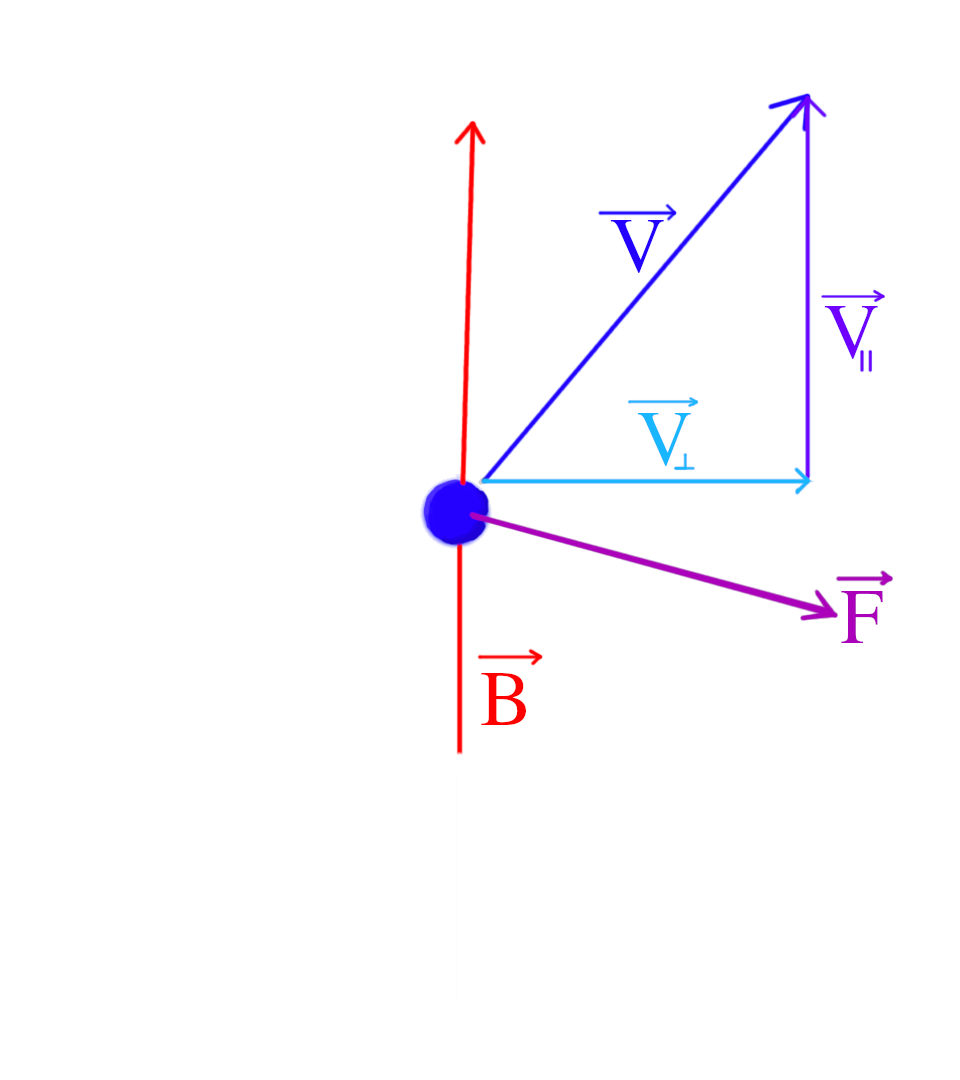
\includegraphics[width=\linewidth]{cyc0.png}}%
%\only<4->{%
%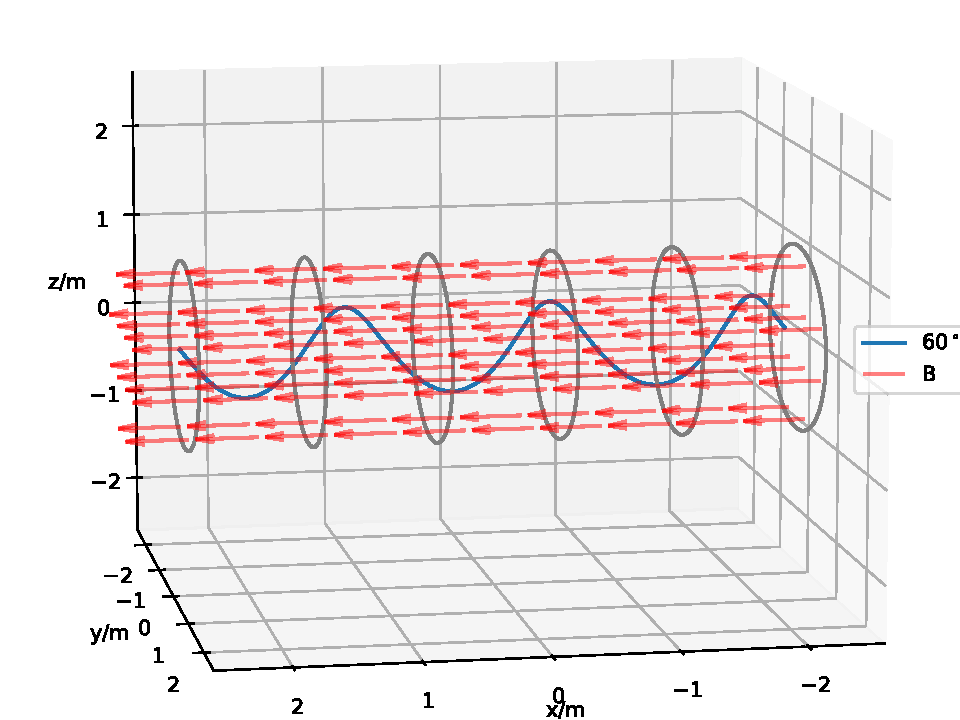
\includegraphics[width=\linewidth]{helix.pdf}}%
\end{column}
\end{columns}
\end{frame}

\begin{frame}
\frametitle{What we expect to see}
\only<1>{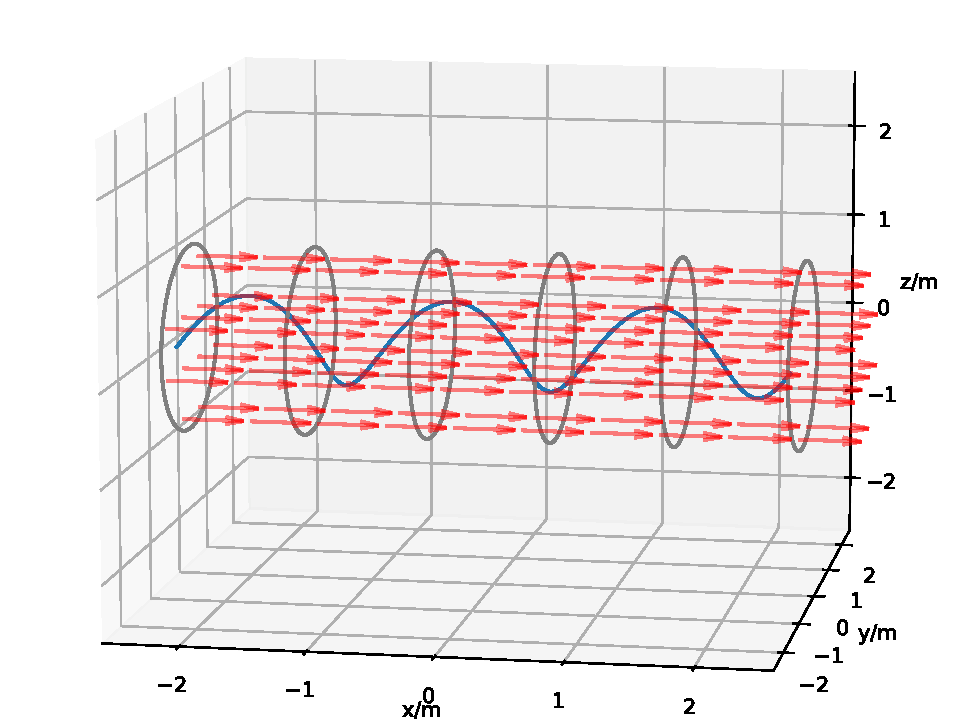
\includegraphics[width=0.8\linewidth]{AN_helix0.pdf}}%
\only<2>{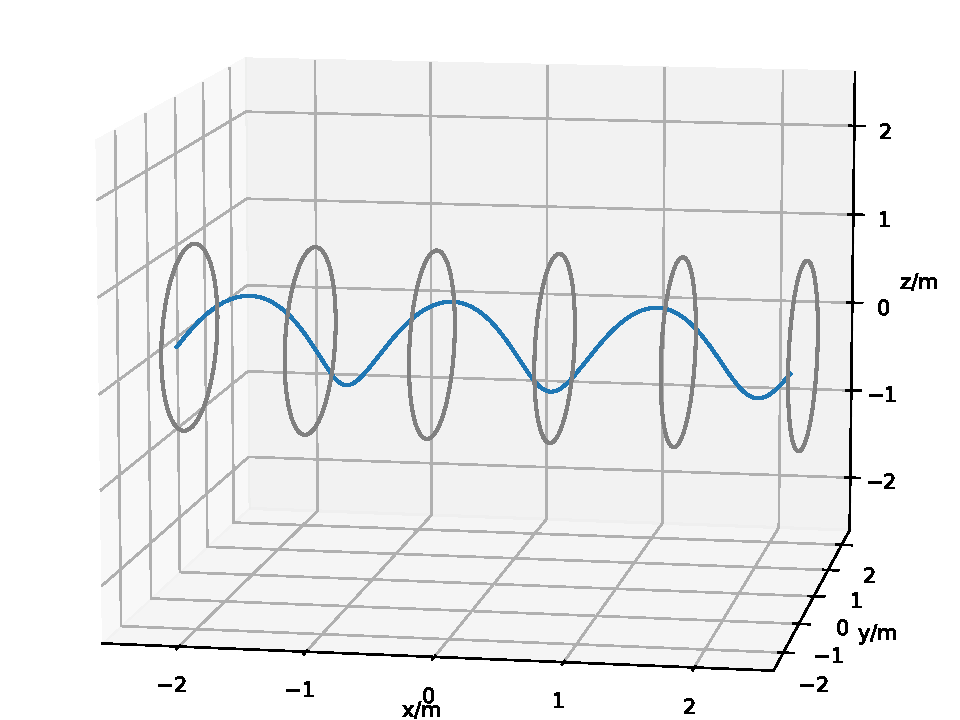
\includegraphics[width=0.8\linewidth]{AN_helix1.pdf}}%
\only<3>{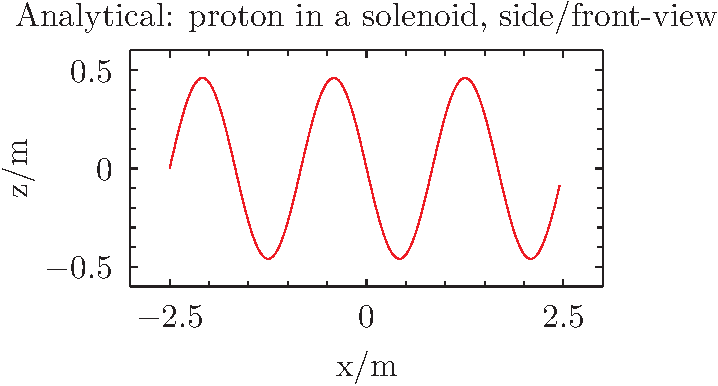
\includegraphics[width=0.66\linewidth]{AN_solenoid_xz_view.pdf}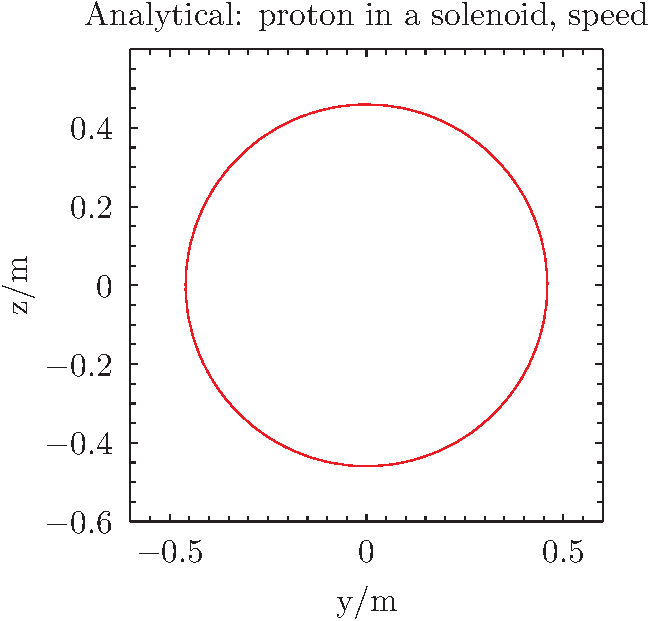
\includegraphics[width=0.33\linewidth]{AN_solenoid_yz_view.pdf}}%
\only<4>{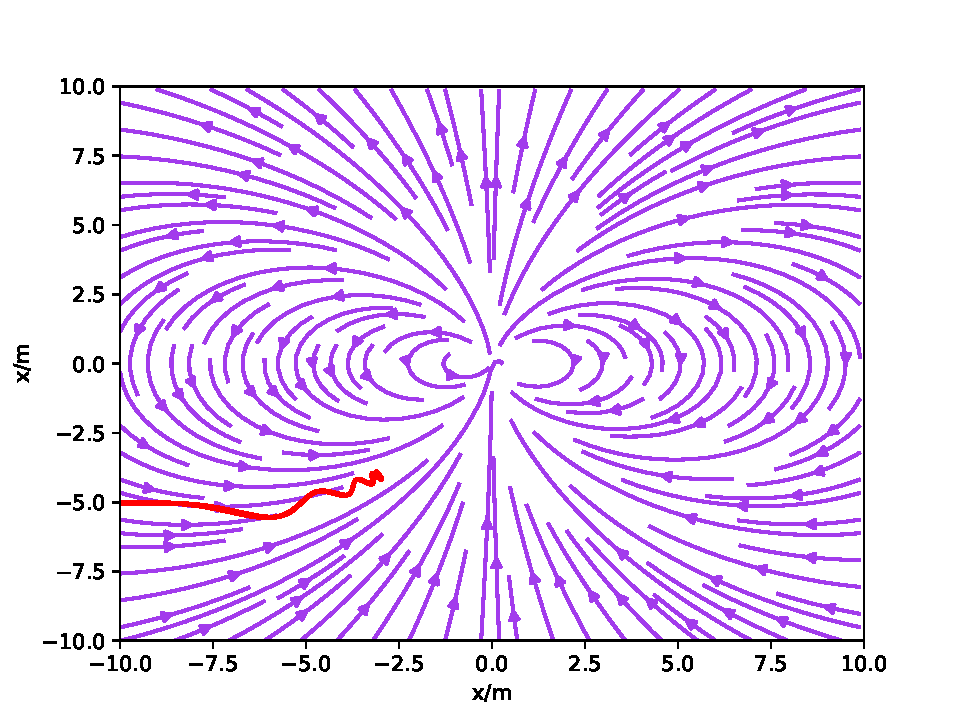
\includegraphics[width=0.8\linewidth]{dipole7.pdf}

(Actually from my simulation)}%

\only<1>{%
``Cyclotron motion"

{\color{gray} Solenoid with $N=1000$ turns per $m$, $I=\SI{5}{\ampere}$, $r=\SI{1}{\meter}$, $|\vec{B}|\approx\SI{6}{\milli\tesla}$. Proton with $E_{kin}=\SI{1}{\mega\electronvolt\per\square\lightspeed}$ ($|v|\approx \SI{3.195E5}{\meter\per\second}$)}}

\only<2-3>{%
``Cyclotron motion"

\begin{equation*}
R \approx \SI{0.5}{\meter}\sin(\theta) \quad T=\frac{2\pi}{\omega_c} \approx \SI{10}{\micro\second}
\end{equation*}
}
\end{frame}

\ifdraft
    \section{Euler's Method and the 4th order Runge-Kutta Method 15 min}
\else
    \section{Euler's Method and the 4th order Runge-Kutta Method}
\fi
%What are they, what are not they

\begin{frame}
\frametitle{Ordinary differential equation's.}
\begin{itemize}
\item<1-> {\color{gray} Sources: Zeigler et al. Theory of Modeling and Simulation (Third edition) chapter 3}

\item<1-> We have:

\begin{align*}
\ddot{\vec{r}}(t) &= \frac{q}{m} ( \dot{\vec{r}}(t)\times \vec{B}(\vec{r},t)+\vec{E}(\vec{r},t)).
\end{align*}

\item<2-> Algorithms exists for ODEs:

\begin{equation*}
\dot{\mathbf{X}} = f_{ode}(\mathbf{X}(t),t).
\end{equation*}


\item<3-> Here:

\begin{align*}
\mathbf{X} = \mvec{\vec{r}}{\dot{\vec{r}}} \quad f_{ode}(\mathbf{X},t) = \mvec{\dot{\vec{r}}}{\frac{q}{m} ( \dot{\vec{r}}\times \vec{B}(\vec{r},t)+\vec{E}(\vec{r},t))}.
\end{align*}
\end{itemize}
\end{frame}

\begin{frame}[fragile]
\frametitle{The ODE to solve}
%\only<1>{%
\begin{lstlisting}
auto ODE = [...](const state_type Data, state_type &dDatadt, const double t){
    //Extract position and velocity from data
    vec pos = vec(Data[0],Data[1],Data[2]);
    vec V = vec(Data[3],Data[4],Data[5]);
    //Lorentz+Newtons 2nd law
    vec F = Charge*(Fields.get_Efield(pos,t)+
        cross(V,Fields.get_Bfield(pos,t)));
    vec dVdt = F*Inv_mass;
    //Save derivative of data
    dDatadt[0]=V.x;dDatadt[1]=V.y;dDatadt[2]=V.z;
    dDatadt[3]=dVdt.x;Datadt[4]=dVdt.y;dDatadt[5]=dVdt.z;
    };
\end{lstlisting}
\end{frame}

\begin{frame}
\frametitle{Ordinary differential equation's.}
\begin{itemize}
\item<1-> {\color{gray} Sources: Zeigler et al. Theory of Modeling and Simulation (Third edition) chapter 3}

\item<1-> We have:

\begin{align*}
\ddot{\vec{r}}(t) &= \frac{q}{m} ( \dot{\vec{r}}(t)\times \vec{B}(\vec{r},t)+\vec{E}(\vec{r},t)).
\end{align*}

\item<1-> Algorithms exists for ODEs:

\begin{equation*}
\dot{\mathbf{X}} = f_{ode}(\mathbf{X}(t),t).
\end{equation*}


\item<1-> Here:

\begin{align*}
\mathbf{X} = \mvec{\vec{r}}{\dot{\vec{r}}} \quad f_{ode}(\mathbf{X},t) = \mvec{\dot{\vec{r}}}{\frac{q}{m} ( \dot{\vec{r}}\times \vec{B}(\vec{r},t)+\vec{E}(\vec{r},t))}.
\end{align*}
\end{itemize}
\end{frame}

\subsection{Euler's Method}

\begin{frame}
\begin{columns}
\begin{column}{0.5\linewidth}
\frametitle{Solving differential equations}
\begin{itemize}

\item<1-> We know only $\mathbf{X}(t_0)$ and $t_0$ and $f_{ode}$.

\item<2-> Can we find $\mathbf{X}(t_0+h)$ for $h>0$?.

\item<3-> Euler's Method:

\begin{equation*}
\mathbf{X}(t_0+h) = \mathbf{X}(t_0)+h f_{ode}(\mathbf{X}(t_0),t_0).
\end{equation*}

\item<3-> Multiple steps $t_0,t_1=t_0+h,\ldots t_i,\ldots$.

\item<4-> Can this be justified?

\item<1-> {\color{gray} Bernard P. Zeigler et al. Theory of Modeling and Simulation (Third edition), chapter 3}
\end{itemize}
\end{column}
\begin{column}{0.5\linewidth}
\only<1-2>{%
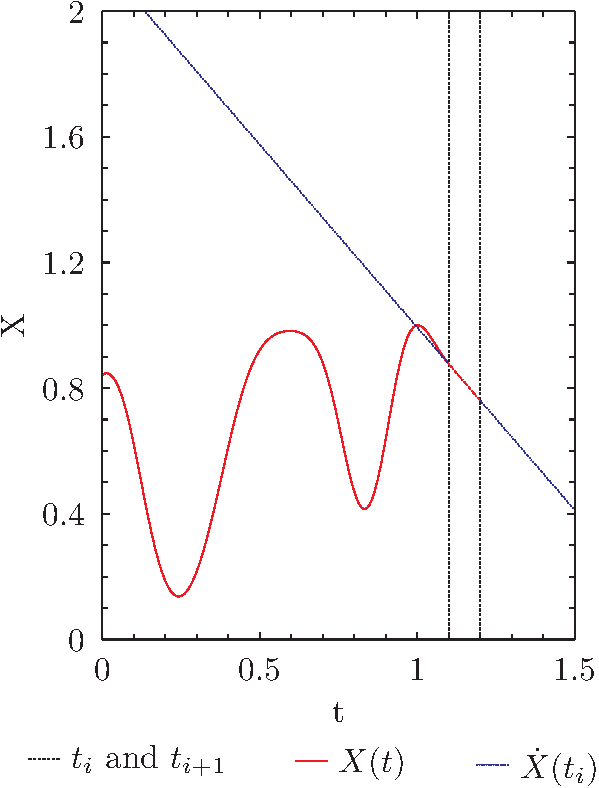
\includegraphics[width=\linewidth]{euler_demo1.pdf}%
}%
\only<3->{%
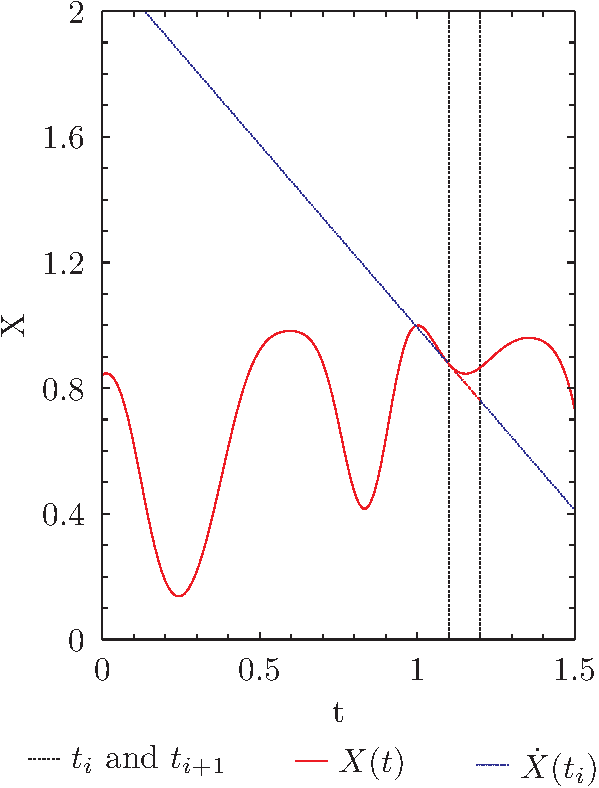
\includegraphics[width=\linewidth]{euler_demo2.pdf}%
}%
\end{column}
\end{columns}
\end{frame}


\begin{frame}
\frametitle{Why does this work? What is the error}
\begin{itemize}
\item<1-> Multiple justifications for why.

\item<2-> First 2 terms in Taylor series {{\color{gray} Zeigler et al.}}:

\begin{equation*}
\only<1>{\mathbf{X}(t_{0}+h) = \mathbf{X}(t_{0})+h \dot{\mathbf{X}}(t_0)+h^2\ldots +\ldots.}
\only<2>{\mathbf{X}(t_{0}+h) = \mathbf{X}(t_{0})+h f_{ode}(\mathbf{X}(t_0),t_0)+h^2\ldots +\ldots.}
\only<3->{\mathbf{X}(t_{i}+h) = \mathbf{X}(t_{i})+h f_{ode}(\mathbf{X}(t_i),t_i)+h^2\ldots +\ldots.}
\end{equation*}

\item<4-> Local error  $~h^2$.

\item<5-> Global error: $~h^1$: All points converges to true path.

\item<6-> We want ``better" (larger $h$  (fewer steps, fewer calls), same error).

\item<7-> Argument suggests we need $\dot{f}_{ode},\ddot{f}_{ode},\ldots$, we don't!
\end{itemize}
\end{frame}

\begin{frame}
\frametitle{The Runge Kutta steppers}
\begin{itemize}

\item<1-> In general:

\begin{equation*}
\mathbf{X}(t_{i+1})-\mathbf{X}(t_{i}) \only<1-3>{=\int_{t_i}^{t_{i+1}}} \only<1>{\dot{\mathbf{X}}(t) dt}\only<2-3>{f_{ode}(\mathbf{X}(t),t) dt }\only<3->{ = h f_{ode}(\mathbf{X}(\tau),\tau)}.
\end{equation*}

\item <3-> \textit{Mean Value theorem for integrals} $t_i\leq \tau\leq t_{i+1}$.

\item<4-> Only possible guess: $\tau=t_i$. Good guess, if $\dot{f}_{ode}\approx 0$.

\item<5-> More generally, (\textit{Explicit} and \textit{single step}), Runge-Kutta family:

\begin{align*}
\mathbf{X}(t_{i+1})-\mathbf{X}(t_{i}) &= \int_{t_i}^{t'} f_{ode}(\mathbf{X}(t),t) dt + \ldots \int_{t^{(m)}}^{t_{i+1}} f_{ode}(\mathbf{X}(t),t) dt \only<6->{,\\ &=  \sum_{j=1}^{m} h_j f_{ode}(\mathbf{X}(\tau_j),\tau_j)}.
\end{align*}

\item<6-> Guess $\tau_1 = t_i$ use $f_{ode}(\mathbf{X}(t_i),t_i)$ to approximate $\mathbf{X}(\tau_2)$ to approximate $\mathbf{X}(\tau_3)$ etc.


\item<1-> {\color{gray} L. Zheng, X. Zhang, Modeling and Analysis of Modern Fluid Problems, 2017, chapter 8}:

\end{itemize}
\end{frame}


\begin{frame}
\frametitle{Runge Kutta methods}
\begin{itemize}

\item<1-> More commonly written:

\begin{equation*}
\mathbf{X}(t_{i+1})-\mathbf{X}(t_{i}) =  h \sum_{j=1}^{m} b_j \mathbf{K}_j
\end{equation*}

\item<2-> Estimate $\mathbf{K}_j$:

\begin{align*}
\mathbf{K}_1 &= f_{ode}(\mathbf{X}(t_i),t_i)\\
\mathbf{K}_2 &= f_{ode}(\mathbf{X}(t_i)+ha_{21} \mathbf{K}_1,t_i+c_2 h)\\
\mathbf{K}_3 &= f_{ode}(\mathbf{X}(t_i)+ha_{31} \mathbf{K}_1+ha_{32} \mathbf{K}_2,t_i+c_3 h)\\
&\vdots
\end{align*}

\item<3-> Want exact for $p$'th order polynomial.

\item<4-> Taylor series analogy: Local error  $~h^{p+1}$, global $~h^{p}$.

\item<1-> {{\color{gray} Martha L. Abell, James P. Braselton, Differential Equations with Mathematica (Fourth Edition), 2016}}:
\end{itemize}
\end{frame}


\begin{frame}
\frametitle{The General explicit Runge Kutta method}
\begin{itemize}


\item<1-> Expressed in Butcher tableu:

\begin{tabular}{l | @{\quad} c @{\quad} c @{\quad} c}
$c_1=0$ \\
$c_2$ & $a_{21}$\\
$c_3$ & $a_{31}$ &  $a_{32}$\\
$c_n$ & $a_{n1}$ &  $a_{n2}$ & $\hdots$\\
\midrule
& $b_1$ & $b_2$ & $\hdots$
\end{tabular}
\end{itemize}
\end{frame}

\subsection{Higher order Runge-Kutta methods}


\begin{frame}
\frametitle{Higher order methods}
\begin{itemize}

\item<1-> 2nd order (Heun's method):

\begin{align*}
\mathbf{X}(t_{i+1})-\mathbf{X}(t_{i}) &= \frac{h}{2}(\mathbf{k}_1+\mathbf{k}_2)\\
\mathbf{k}_1 &= f_{ode}(\mathbf{X}(t_i),t_i)\\
\mathbf{k}_2 &= f_{ode}(\mathbf{X}(t_i)+h\mathbf{k}_1,t_i+h).
\end{align*}

\end{itemize}
\end{frame}

\begin{frame}
\frametitle{Higher order methods}
\begin{columns}
\begin{column}{0.5\linewidth}
\begin{itemize}
\item<1-> 4th order, often simply called the Runge Kutta method:

\begin{align*}
\mathbf{X}(t_{i+1})-\mathbf{X}(t_{i}) &= \frac{h}{6}(\mathbf{k}_1+2\mathbf{k}_2+2\mathbf{k}_3+\mathbf{k}_4 )\\
\mathbf{k}_1 &= f_{ode}(\mathbf{X}(t_i),t_i)\\
\mathbf{k}_2 &= f_{ode}(\mathbf{X}(t_i)+\frac{h}{2}\mathbf{k}_1,t_i+\frac{h}{2})\\
\mathbf{k}_3 &= f_{ode}(\mathbf{X}(t_i)+\frac{h}{2}\mathbf{k}_2,t_i+\frac{h}{2})\\
\mathbf{k}_4 &= f_{ode}(\mathbf{X}(t_i)+h\mathbf{k}_3,t_i+h).
\end{align*}

\end{itemize}
\end{column}
\begin{column}{0.5\linewidth}
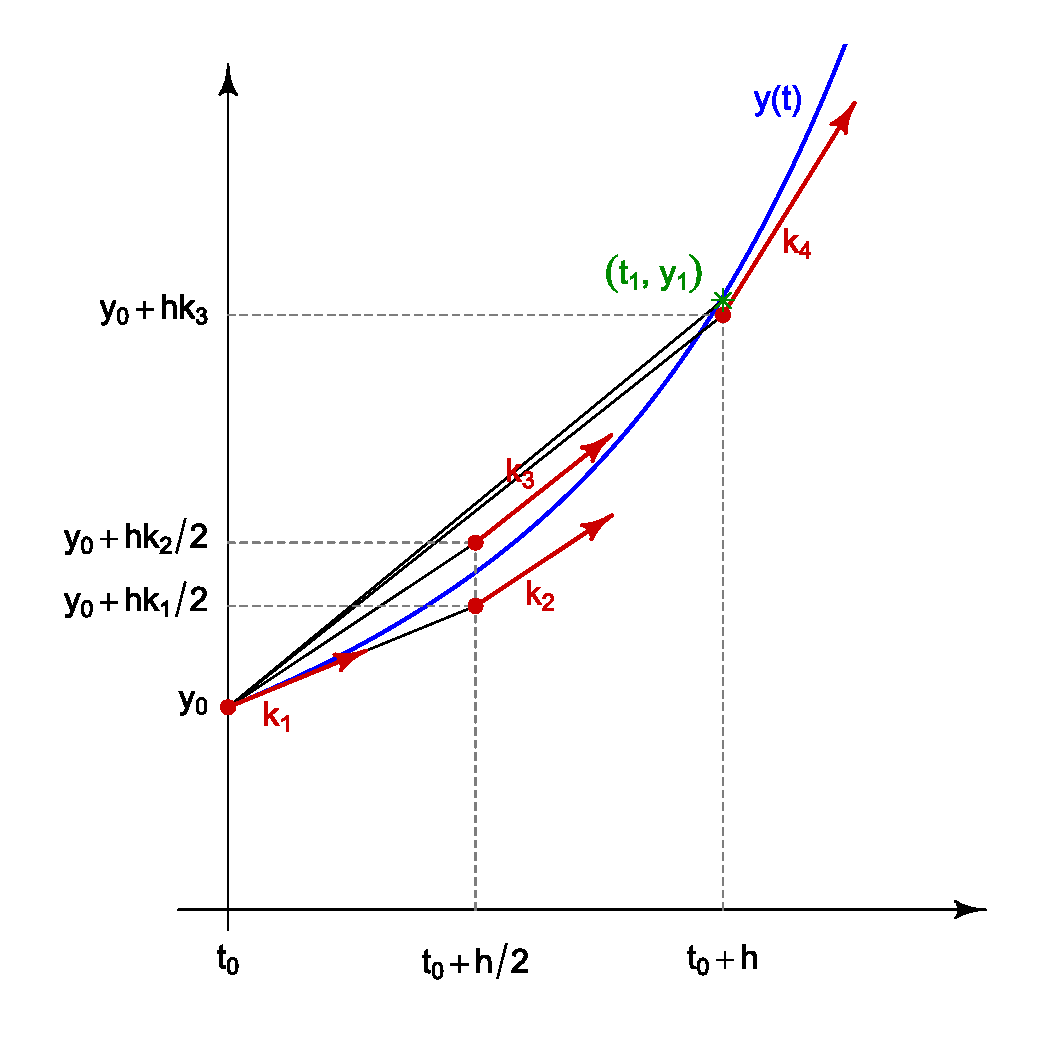
\includegraphics[width=\linewidth]{Runge-Kutta_slopes.pdf}

{\color{gray} Wikipedia-user HilberTraum, published under creative commins: CC BY-SA 4.0}
\end{column}
\end{columns}
\end{frame}

\begin{frame}[fragile]
\frametitle{Euler Implementations}
\begin{lstlisting}
state_type Data = Data0;
state_type dDatadt;
size_t time_res = T/timestep;
for (size_t i = 1; i < time_res; ++i)
{
    double t=i*dt;
    ODE(Data,dDatadt,t);
    //Euler time evolution
    Data+=timestep*dDatadt;

    save_step( Data , i*timestep );
};
\end{lstlisting}
\end{frame}

\begin{frame}[fragile]
\frametitle{RK4 Implementations (1/2)}
\begin{lstlisting}
state_type Data = Data0;
state_type temp=Data0;
state_type K1,K2,K3,K4;
size_t time_res = T/timestep;
for (size_t i = 1; i < time_res; ++i)
{
    double t=i*timestep;

    //substep 1
    ODE(Data,K1,t);

    //substep 2
    temp=Data+timestep*K1/2;
    ODE(temp,K2,t+timestep/2);
\end{lstlisting}
\end{frame}

\begin{frame}[fragile]
\frametitle{RK4 Implementations (2/2)}
\begin{lstlisting}

    //substep 3
    temp=Data+timestep*K2/2;
    ODE(temp,K3,t+timestep/2);

    //substep 4
    temp=Data+timestep*K3;
    ODE(temp,K4,t+timestep);

    //Read data
    Data+=timestep*(K1+2.0*K2+2.0*K3+K4)/6.0;
    save_step( Data , i*timestep );}
}
\end{lstlisting}
\end{frame}


%\begin{frame}[fragile]
%\frametitle{``Correct" way}
%\begin{lstlisting}
%#include <boost/array.hpp>
%#include <boost/numeric/odeint.hpp>
%using namespace boost::numeric::odeint;
%typedef boost::array< double, 6 > state_type;
%...
%size_t steps = integrate_const(
%    runge_kutta4< state_type >(),
%    ODE,   //Lorentz-force
%    Data0 ,//{pos0,v0}
%    0.0 ,  //t0=0
%    T ,    //max time
%    timestep ,//length of each step
%    save_step //User defined save data function
%);
%\end{lstlisting}
%\end{frame}

\subsection{Demonstration, particles in a solenoid}

\begin{frame}
\frametitle{Does it work}
\begin{itemize}

\item<1-> Test, same proton in a solenoid use $\theta=\ang{60}$ reference, had:

\begin{equation*}
R \approx \SI{0.5}{\meter}\sin(\theta)\approx \SI{0.45}{\meter} \quad T=\frac{2\pi}{\omega_c} \approx \SI{10}{\micro\second}.
\end{equation*}

\item<2-> Compare Analytic, Euler, Runge-Kutta 4.

\item<3-> Consider $\theta=\ang{60}$ at different $h$.

\item<4-> Check error on $|\vec{v}|$, $R=\sqrt{y^2+z^2}$.
\end{itemize}
\end{frame}


\makeatletter
\begin{frame}
\frametitle{At a glance, 3D view}
    \global\beamer@shrinktrue
    \gdef\beamer@shrinkframebox{
        \setbox\beamer@framebox=\vbox to\beamer@frametextheight{
            \centering
            $h=t_{i+1}-t_i=\SI{0.01}{\micro\second}$

            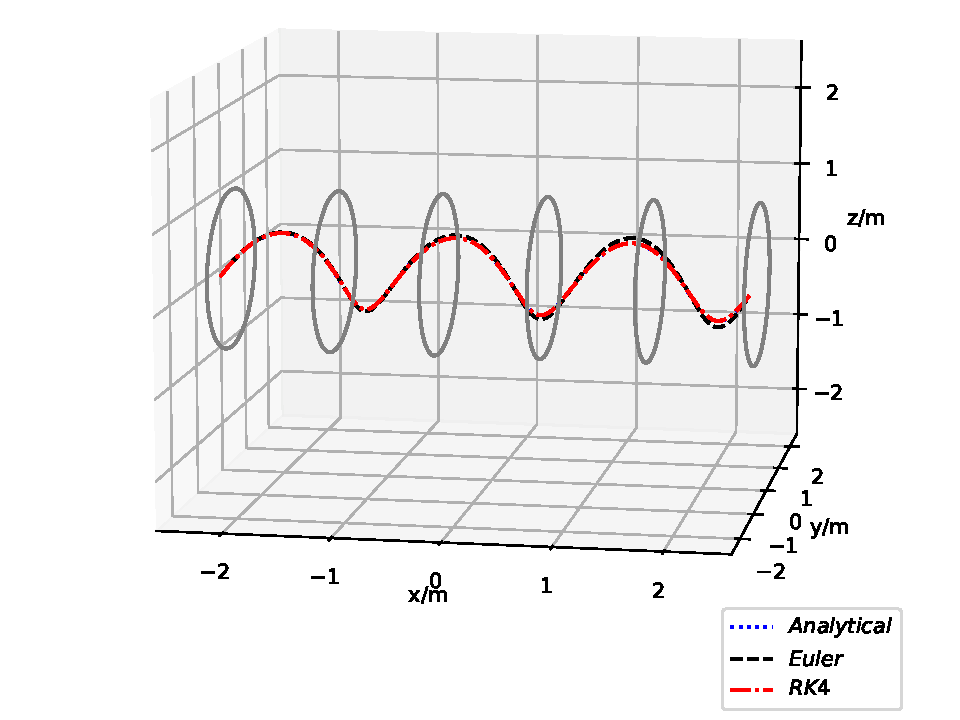
\includegraphics[height=0.9\beamer@frametextheight]{Solenoid_compare001_3D.pdf}

            3129 steps
        }
    }
\end{frame}
\makeatother

\makeatletter
\begin{frame}
\frametitle{At a glance, 3D view}
    \global\beamer@shrinktrue
    \gdef\beamer@shrinkframebox{
        \setbox\beamer@framebox=\vbox to\beamer@frametextheight{
            \centering
            $h=t_{i+1}-t_i=\SI{0.1}{\micro\second}$

            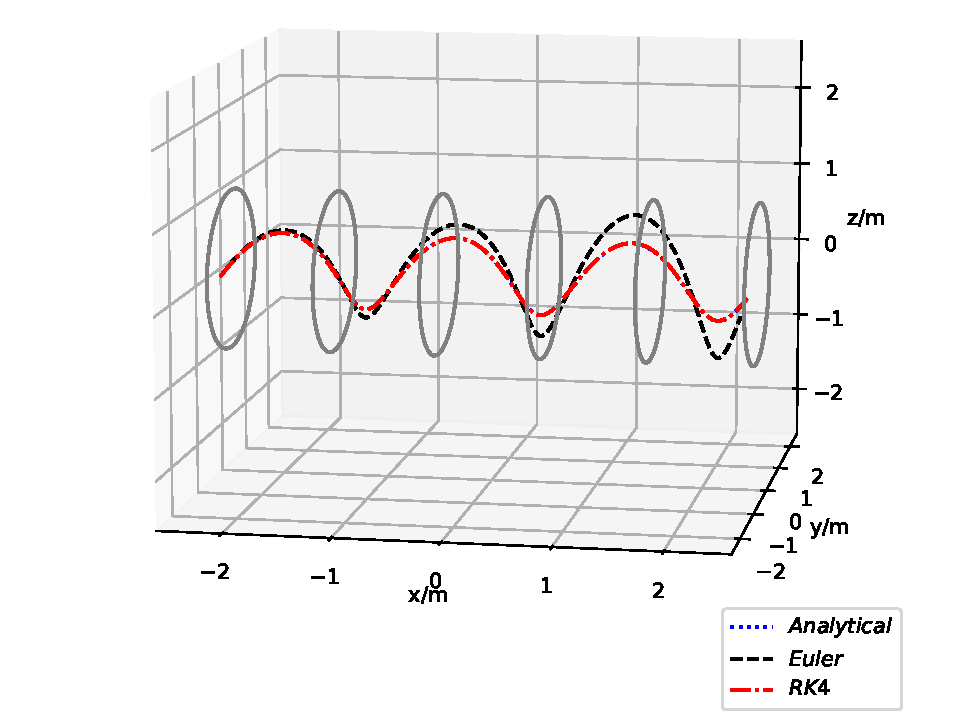
\includegraphics[height=0.9\beamer@frametextheight]{Solenoid_compare01_3D.pdf}

            312 steps
        }
    }
\end{frame}
\makeatother

\makeatletter
\begin{frame}
\frametitle{At a glance, 3D view}
    \global\beamer@shrinktrue
    \gdef\beamer@shrinkframebox{
        \setbox\beamer@framebox=\vbox to\beamer@frametextheight{
            \centering
            $h=t_{i+1}-t_i=\SI{1.0}{\micro\second}$

            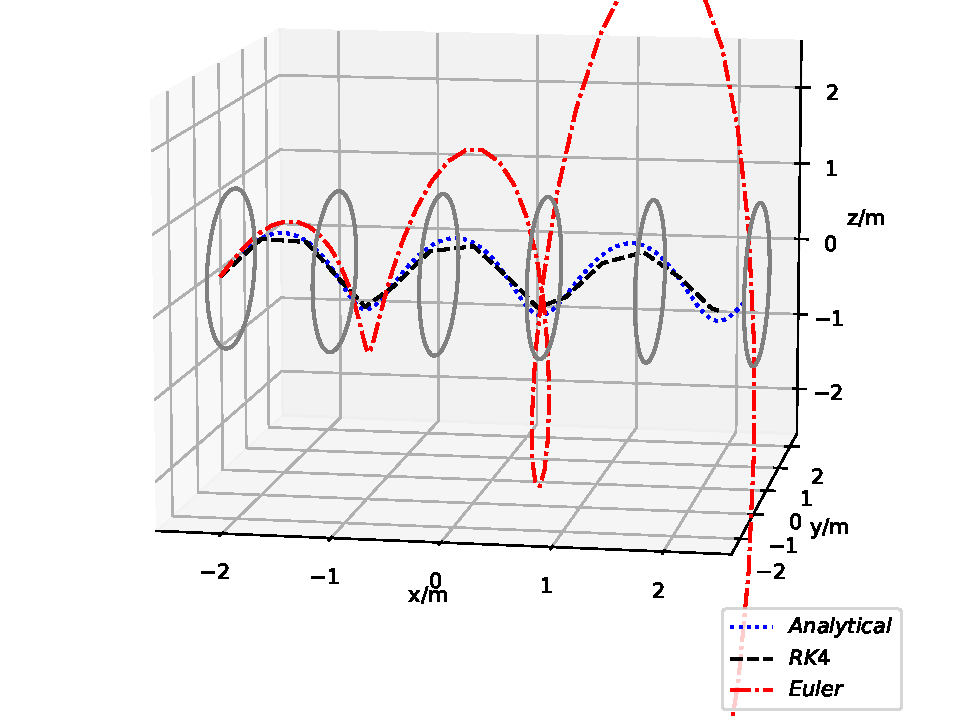
\includegraphics[height=0.9\beamer@frametextheight]{Solenoid_compare1_3D.pdf}

            31 steps.
        }
    }
\end{frame}
\makeatother

\begin{frame}
\frametitle{At a glance, front view, no border}
\only<1>{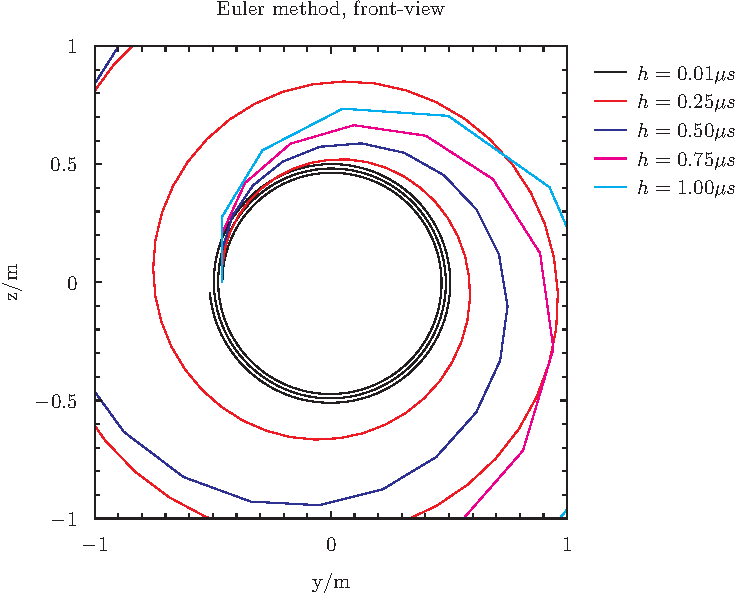
\includegraphics[width=\linewidth]{solenoid_euler_yz_view.pdf}}%
\only<2>{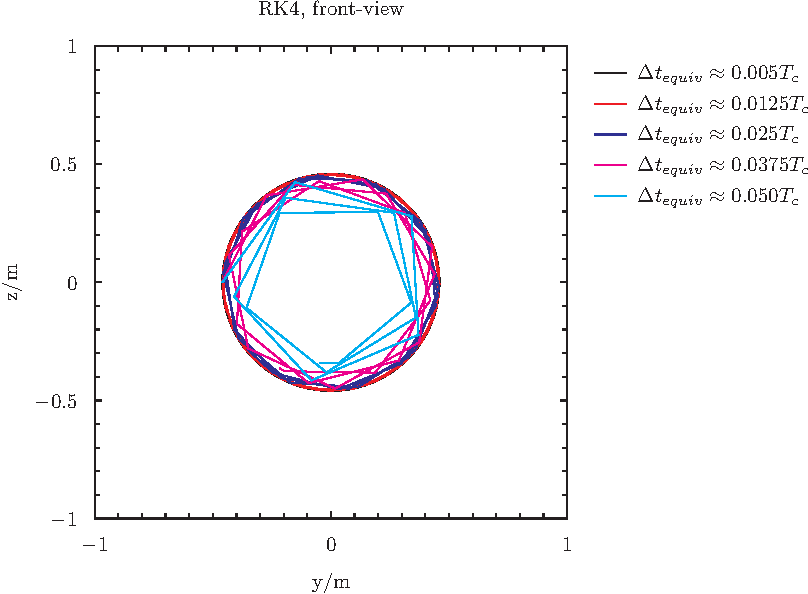
\includegraphics[width=\linewidth]{solenoid_RK_yz_view.pdf}}
\end{frame}

\begin{frame}
\frametitle{Constant radius?}
\only<1>{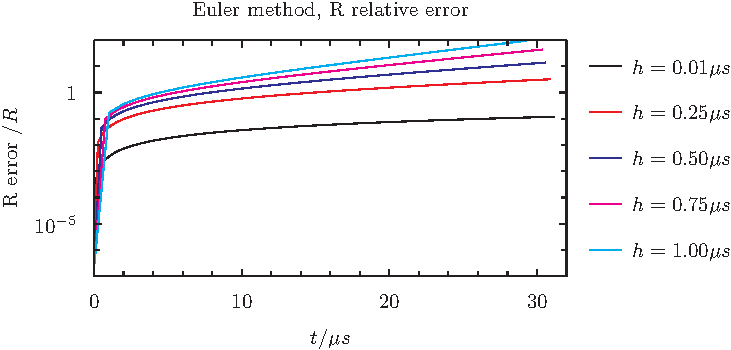
\includegraphics[width=\linewidth]{solenoid_euler_Rt.pdf}}%
\only<2>{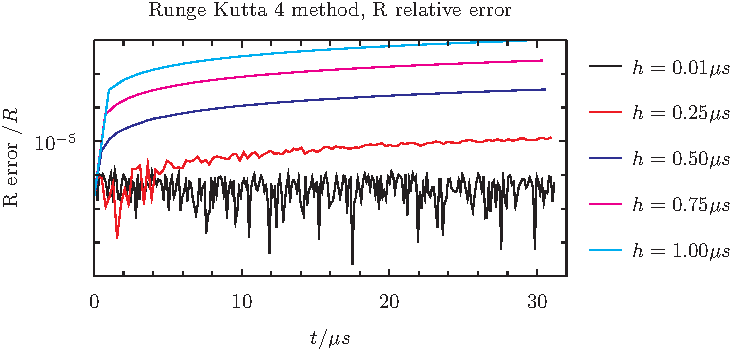
\includegraphics[width=\linewidth]{solenoid_RK4_Rt.pdf}}
\end{frame}


\begin{frame}
\frametitle{Error as function of $h$}
\only<1>{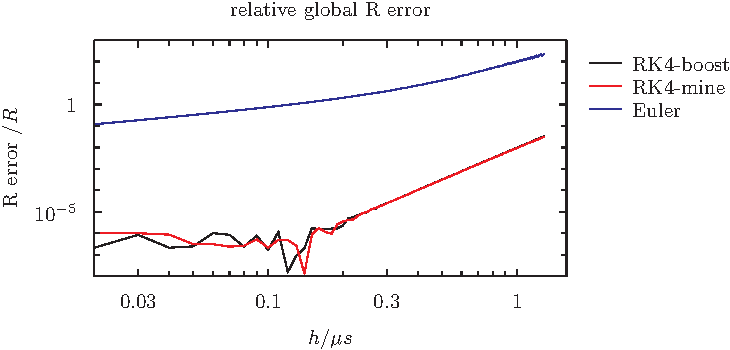
\includegraphics[width=\linewidth]{solenoid_Rh.pdf}}%
\end{frame}


\ifdraft
    \section{Embedded algorithms, and adaptive step size 15 min}
\else
    \section{Embedded algorithms, and adaptive step size}
\fi


\begin{frame}
\frametitle{What is not to like?}

\begin{columns}
\begin{column}{0.5\linewidth}
\begin{itemize}
\item <2-> Usually don't know error.

\item <2-> Hard to pick $h$ , and may change:

\item <3-> Inhomogeneous fields (here, a true dipole)

\item <4-> Time dependent fields (here the cyclotron, bad example)

\item <5-> Let the computer pick $h$ for error.

\end{itemize}
\end{column}
\begin{column}{0.5\linewidth}


\only<3,5>{%
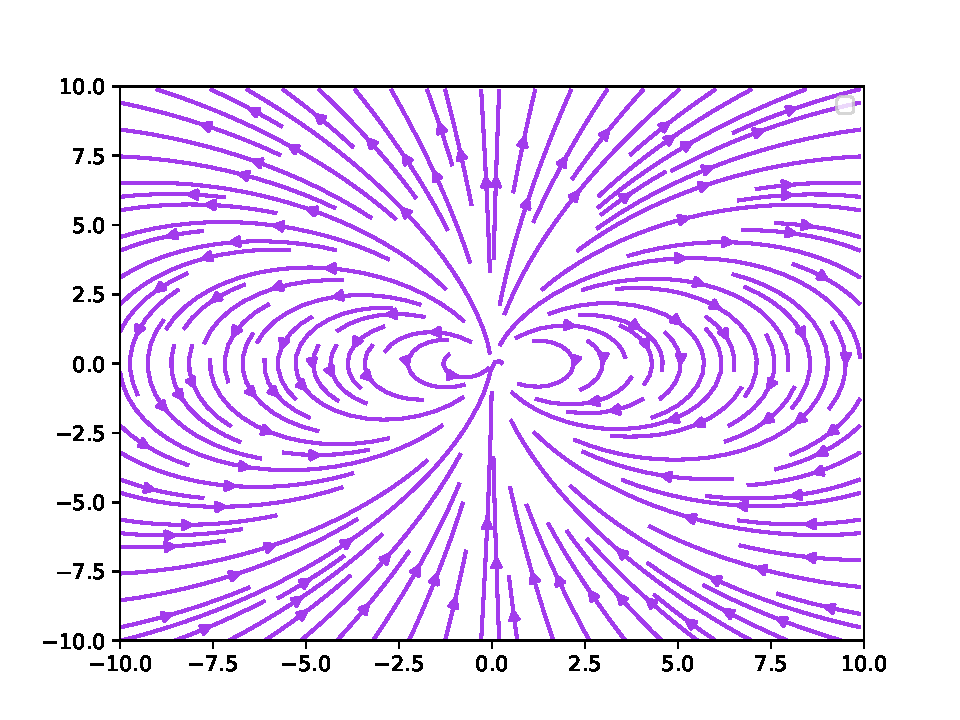
\includegraphics[width=\linewidth]{dipole.pdf}

}%


\only<4>{%
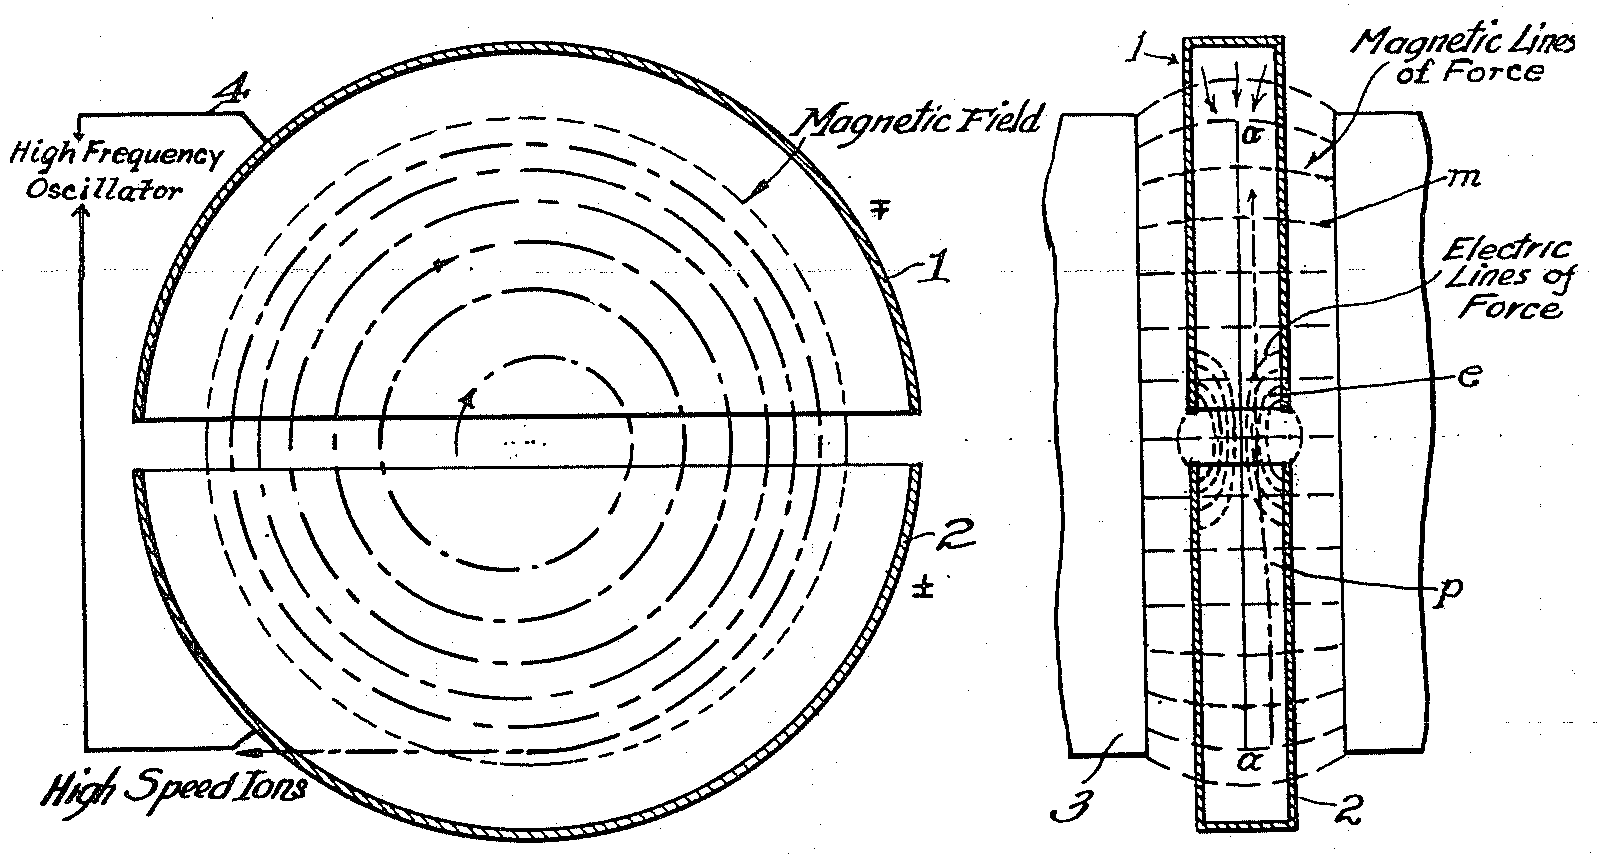
\includegraphics[width=\linewidth]{ Cyclotron_patent.png}

{\color{gray} Ernest O. Lawrence, 1934, U.S. Patent 1,948,384; image in Public Domain.}
}%

\end{column}
\end{columns}
\end{frame}


\begin{frame}
\frametitle{Example, magnetic dipole}

\begin{columns}
\begin{column}{0.5\linewidth}
\begin{itemize}

\item <1-> True dipole:

\begin{align*}
\vec{B} = \frac{\mu_0}{4\pi r^3} \left[3 \hat{\vec{r}}(\vec{m}\cdot\hat{\vec{r}} -\vec{m}) \right].
\end{align*}

\item <2-> Weak field, little change, long steps.

\item <3-> strong field, large change, short steps.

\item <4-> No analytical solution.


\end{itemize}
\end{column}
\begin{column}{0.5\linewidth}


\only<1>{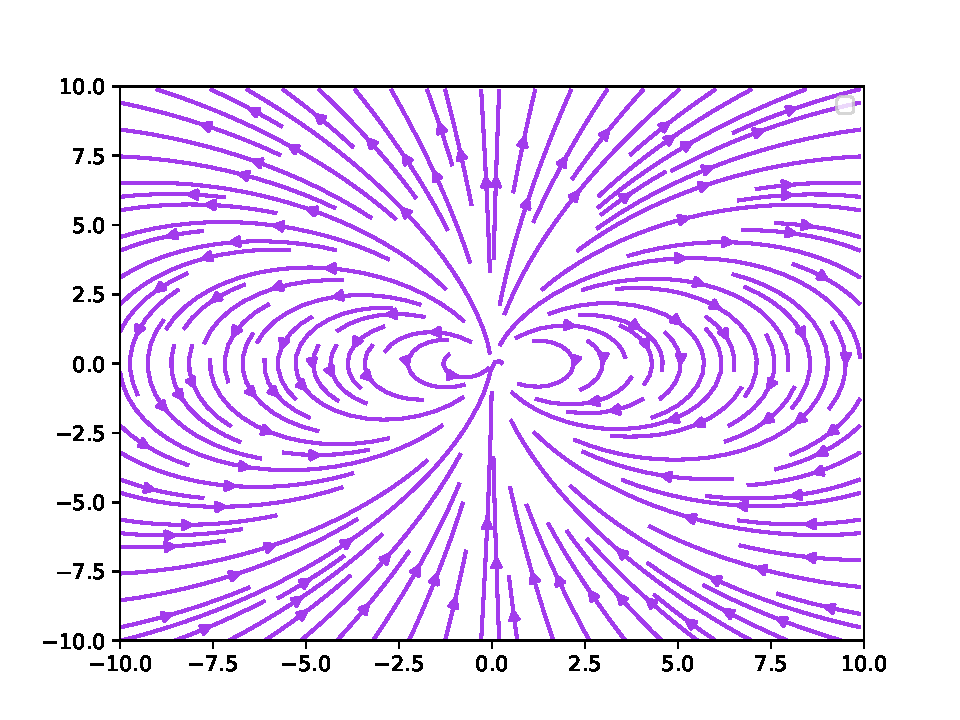
\includegraphics[width=\linewidth]{dipole.pdf}}%
\only<2->{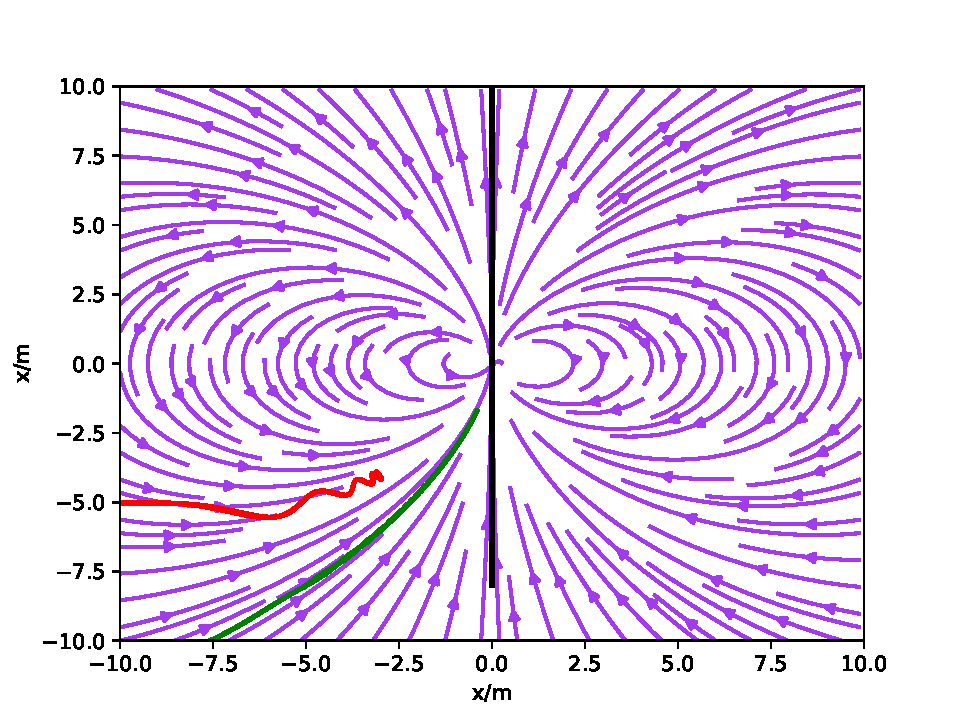
\includegraphics[width=\linewidth]{dipole6.pdf}

{\color{gray}  Arbitrarily set $\frac{\mu_0}{4\pi}|\vec{m}|= \SI{0.155}{\tesla\per\cubic\meter}$ .

 Protons with speed around $\SI{10000}{\meter\per\second}$}


}%
\end{column}
\end{columns}
\end{frame}


\subsection{Dormand Prince 5 (4) method}

\begin{frame}
\frametitle{Embedded Runge-Kutta algorithms}
\begin{itemize}
\item <1-> Need estimate for error.

\item <2-> Runge-Kutta step $\mathbf{X}^{(p)}(t_{i+1})$ will converge to $\mathbf{X}(t_{i+1})$.
\item <3-> Use 2 different order methods, $\mathbf{X}^{(p-1)}(t_{i+1})$, $\mathbf{X}^{(p)}(t_{i+1})$.

\item <4-> Approximate ``Error" as  $\mathbf{E}_j = |\mathbf{X}^{(p-1)}_j(t_{i+1})-\mathbf{X}^{(p)}_j(t_{i+1})|$.

\item <5-> Adjust step size to keep the error(s) small (Implementations differ!).

{\color{gray} Dormand, J. R.; Prince, P. J. (1980), "A family of embedded Runge-Kutta formulae", Journal of Computational and AppliMathematics}
\begin{equation}
\end{equation}


\end{itemize}
\end{frame}


\begin{frame}
\frametitle{Runge-Kutta Dormand Prince 5 (4)}

\begin{itemize}
\item <1->\lstinline{ode45} in Matlab, \lstinline{scipy.solve_ivp} in Python , \lstinline{RungeKutta_dopri5} in \lstinline{boost::odeint}.

\begin{align*}
\mathbf{X}^{(5)}(t_{i+1})-\mathbf{X}(t_{i}) &=  h \sum_{j=1}^{m} b_j^{(5)} \mathbf{k}_j\\
\mathbf{X}^{(4)}(t_{i+1})-\mathbf{X}(t_{i}) &=  h \sum_{j=1}^{m} b_j^{(4)} \mathbf{k}_j.
\end{align*}

\begin{align*}
\mathbf{k}_j &= f_{ode}(\mathbf{X}(t_i)+h \sum_k^{j-1} a_{kj} \mathbf{k}_j,t_i+c_3 h).
\end{align*}

\item <2-> 7 $\mathbf{k}_j$'s (actually 6 by clever re-usage).

{\color{gray} Dormand, J. R.; Prince, P. J. (1980), "A family of embedded Runge-Kutta formulae", Journal of Computational and Applied Mathematics}
\end{itemize}
\end{frame}

\begin{frame}
\frametitle{Butcher Tableu of Dormand Prince (5) 4}
\begin{tabular}{c | @{\quad} c @{\quad} c @{\quad} c @{\quad} c @{\quad} c @{\quad} c @{\quad} c @{\quad} c}
$c_i$ & $a_{ij}$ & $\hdots$\\
\midrule
$0$ \\
$\frac{1}{5}$ & $\frac{1}{5}$\\
$\frac{3}{10}$ & $\frac{3}{40}$ &  $\frac{9}{40}$\\
$\frac{4}{5}$ & $\frac{40}{45}$ &  $-\frac{56}{15}$  &  $-\frac{32}{9}$\\
$\frac{8}{9}$ & $\frac{19372}{6561}$ & $-\frac{25360}{2187}$ & $\frac{64448}{6561}$ & $-\frac{212}{729}$\\
$1$ & $\frac{9017}{3168}$ & $-\frac{355}{33}$ & $\frac{46732}{5247}$ & $\frac{49}{176}$  & $-\frac{5103}{18656}$\\
$1$ & $\frac{35}{384}$  & $0$	 & $\frac{500}{1113}$ & $\frac{125}{192}$ & $-\frac{2187}{6784}$ & $\frac{11}{84}$\\
\midrule
$/b^{(5)}$  & $\frac{35}{384}$ & $0$ & $\frac{500}{1113}$ & $\frac{125}{192}$ & $-\frac{2187}{6784}$ & $\frac{11}{84}$ & $0$\\
$/b^{(4)}$ & $\frac{5179}{57600}$ & $0$ & $\frac{7571}{16695}$ & & $\frac{393}{640}$ & $-\frac{92097}{339200}$& $\frac{187}{2100}$ & $\frac{1}{40}$
\end{tabular}
\end{frame}

\begin{frame}
\frametitle{Runge-Kutta Dormand Prince 5 (4)}

\begin{itemize}
\item <1-> Step size correction (Dormand Prince):

\begin{align*}
h_{new} = 0.9 h_{old} \left[\frac{\delta }{||\mathrm{E}||}\right]^{\frac{1}{p+1}}
\end{align*}

\item <2-> Step size correction (Me):

\begin{align*}
h_{new} &= \min_j \left(0.9 h_{old} \left[\frac{\delta_j}{\mathrm{E}_{j}}\right]^{\frac{1}{p}}\right), \quad \mathrm{E}_j>\delta_j : \mathrm{reject}\\
\delta_j &=\min(\delta_{abs},|\mathbf{X}_j(t_{i})|\delta_{rel})\sqrt{\frac{h_{old}}{T}}.
\end{align*}

\item <3-> Scale by step size $\frac{h_{old}}{T}$, ``Fail safe" $\sqrt{\ldots}$.

{\color{gray} Dormand, J. R.; Prince, P. J. (1980), "A family of embedded Runge-Kutta formulae", Journal of Computational and Applied Mathematics}
\end{itemize}
\end{frame}

\subsection{Demonstration: magnetic dipole}

\begin{frame}
\frametitle{Does it work?}
\begin{centering}
\only<1>{%
\noindent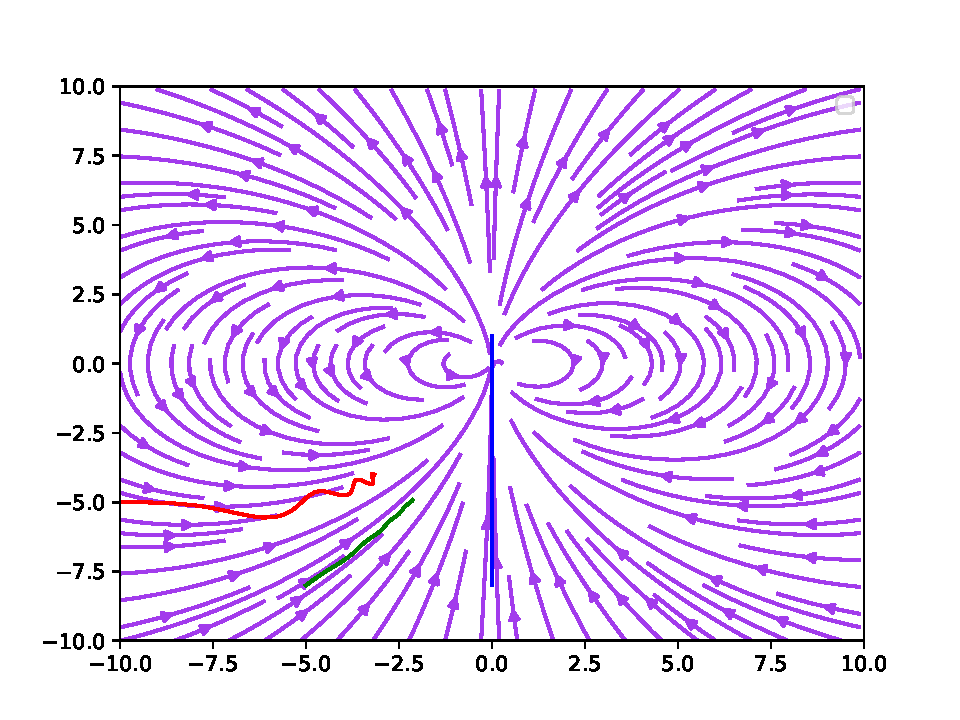
\includegraphics[width=0.8\linewidth]{dipole2.pdf}

My version relative and absolute error $10^{-6}$. 94 steps (+ 14 rejected).
}%
\only<2>{%
\noindent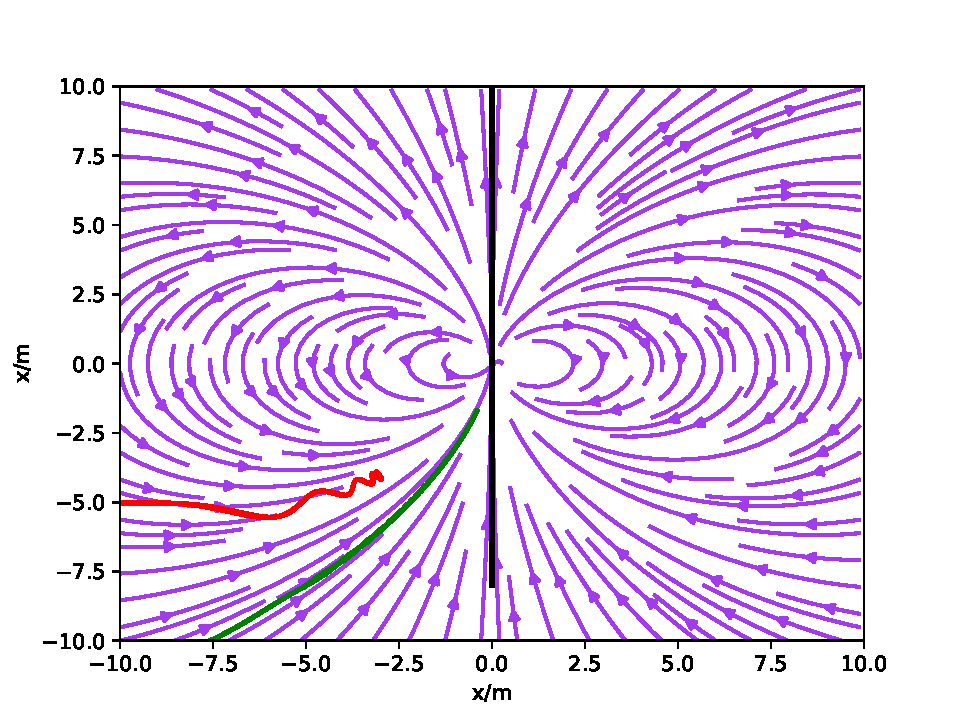
\includegraphics[width=0.8\linewidth]{dipole3.pdf}

Odeint library relative and absolute error $10^{-7}$. 92 steps.
}%
\only<3>{%
\noindent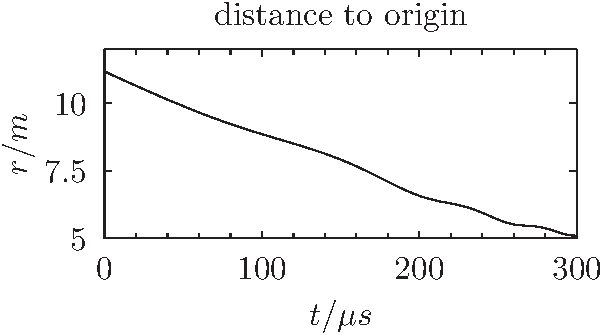
\includegraphics[width=\linewidth]{dipole_R.pdf}}%
\only<4>{%
\noindent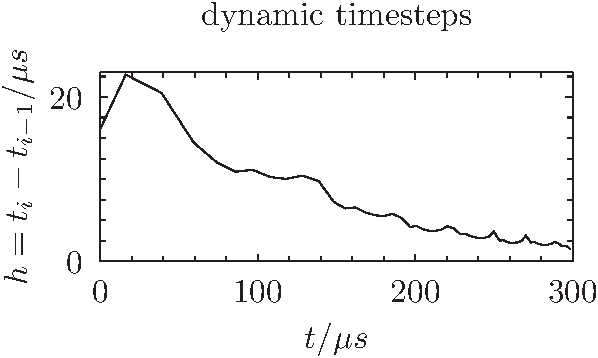
\includegraphics[width=\linewidth]{dipole_h.pdf}

My version, adaptive step size.
}%



\end{centering}
\end{frame}


\begin{frame}
\frametitle{Another curious result}
\begin{centering}
\only<1>{%
\noindent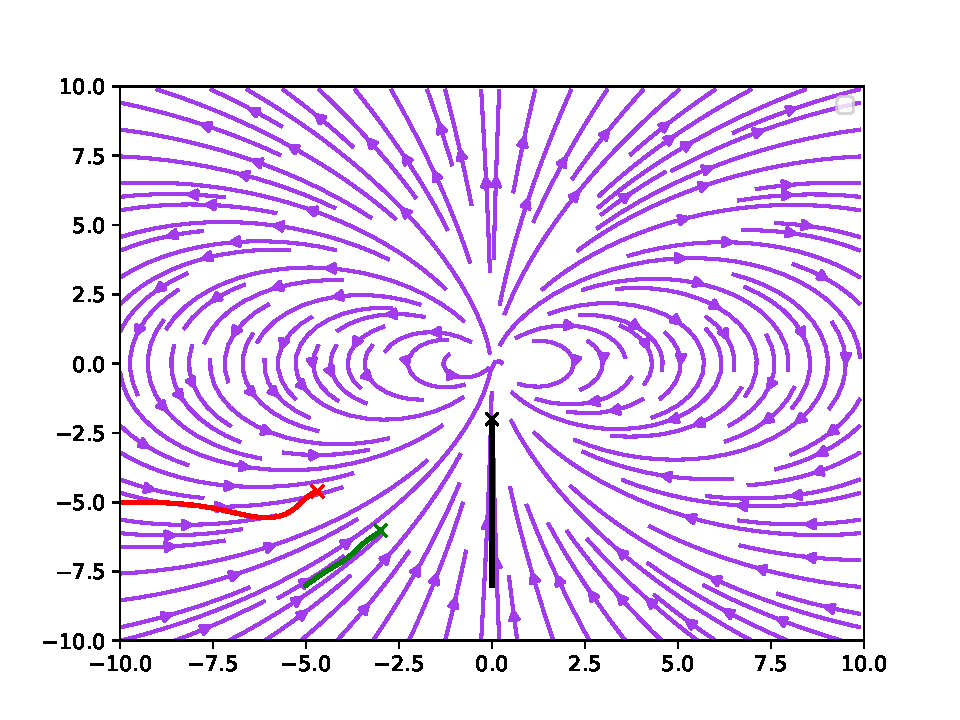
\includegraphics[width=0.8\linewidth]{dipole4.pdf}

$T = \SI{0.2}{\milli\second}$
}
\only<2>{%
\noindent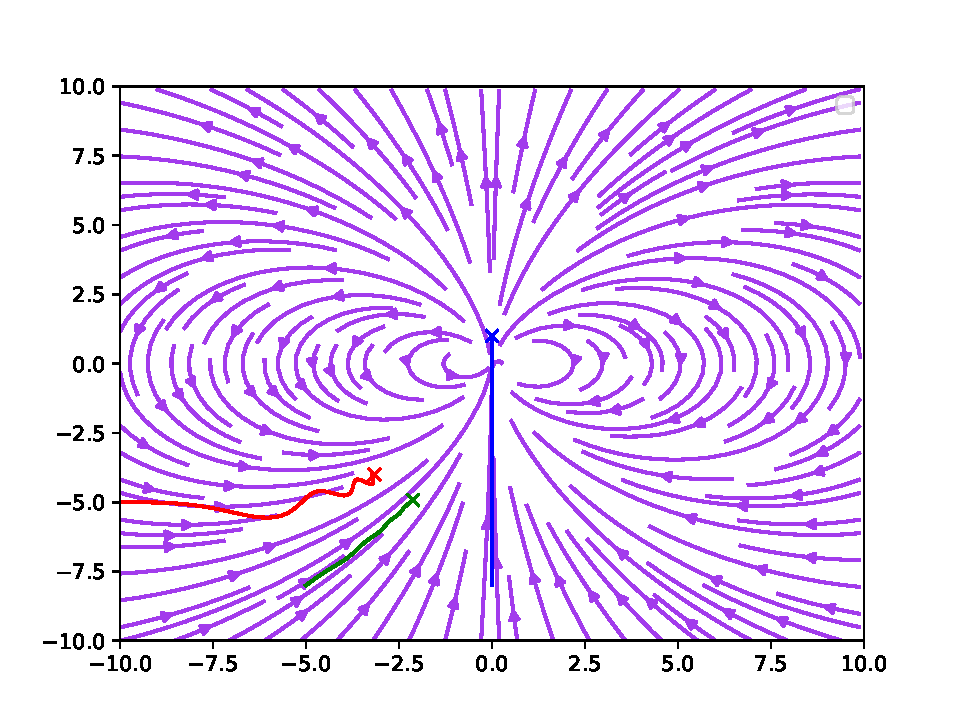
\includegraphics[width=0.8\linewidth]{dipole5.pdf}

$T = \SI{0.3}{\milli\second}$

}%
\only<3>{%
\noindent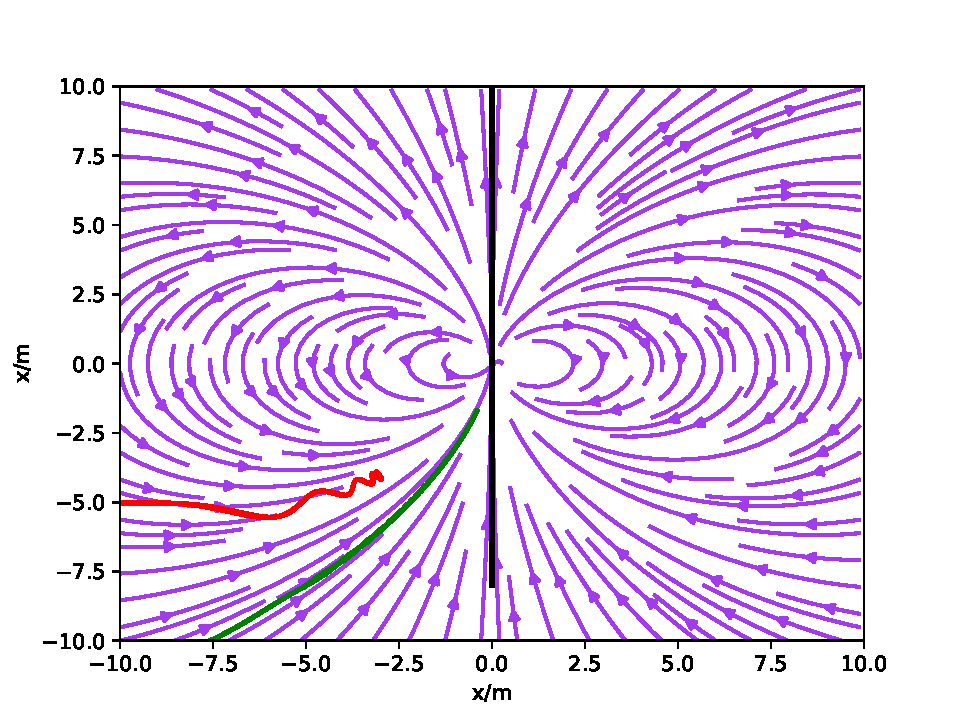
\includegraphics[width=0.8\linewidth]{dipole6.pdf}

$T = \SI{0.6}{\milli\second}$

Magnetic ``mirror" or ``bottle".
}%
\only<4>{%
\noindent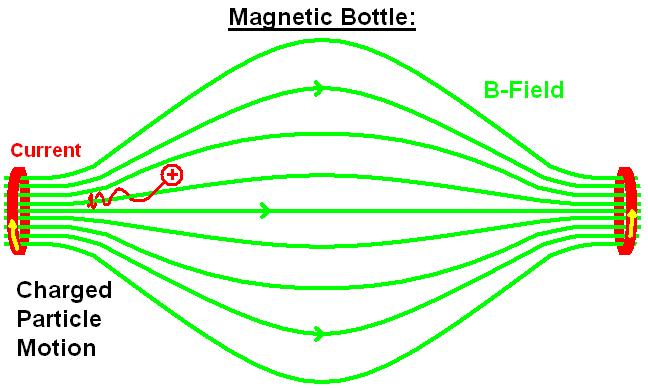
\includegraphics[width=\linewidth]{Fields_in_magnetic_bottles.jpg}

{\color{gray} Wikipedia user WikiHelper2134 , Public Domain.}
}%
\only<5>{%
\noindent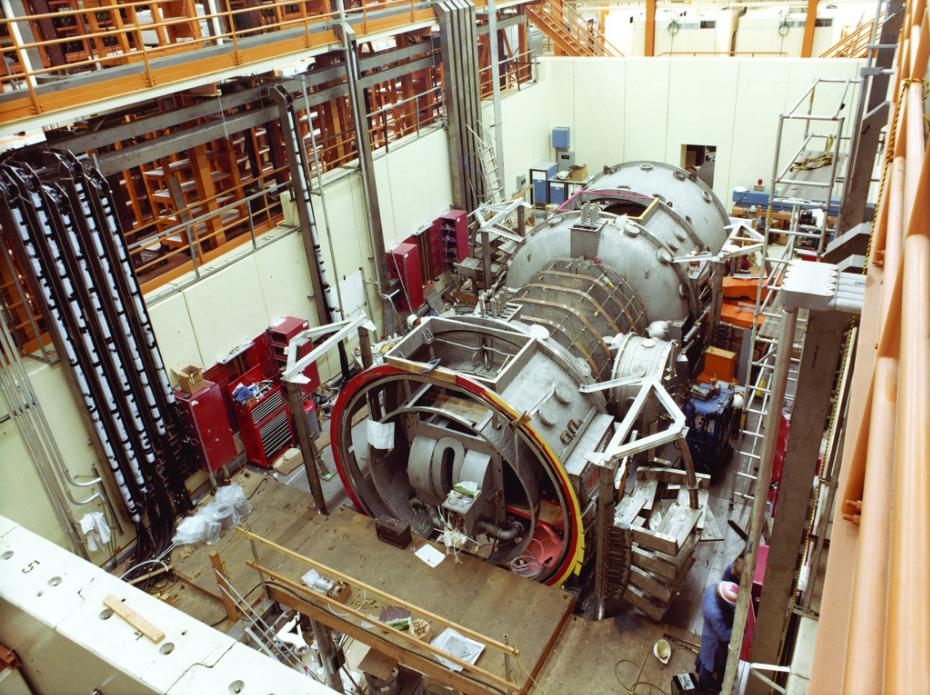
\includegraphics[width=0.8\linewidth]{magnetic_bottles.jpg}

{\color{gray} Tandem Mirror Experiment, The Lawrence Livermore National Laboratory, 1978.}

}%
\end{centering}
\end{frame}


\section{Conclusion}

\begin{frame}
\frametitle{Conclusion }
\begin{itemize}
\item<1-> Simulating particles in electric and magnetic fields.
\item<2-> Numerically solving ordinary differential equations
\item<2-> Reasonable agreement with known results.
\item<2-> Can easily be generalized to other systems.
\item<3-> Limitation, simulations are not experiments.
\end{itemize}
\end{frame}

%\subsection{If time permits, the cyclotron}

\begin{frame}
\frametitle{Example, cyclotron}
\begin{columns}
\begin{column}{0.5\linewidth}
\begin{itemize}
\item<1-> Electric field accelerates, magnetic contains.

\item<2-> Single gab, oscillating field.

\item<3-> Uses classical Cyclotron frequency

\item<4-> Analytical final speed, in principle path.

\begin{equation*}
\frac{R|q|B}{m} = v_\perp
\end{equation*}

\end{itemize}
\end{column}
\begin{column}{0.5\linewidth}
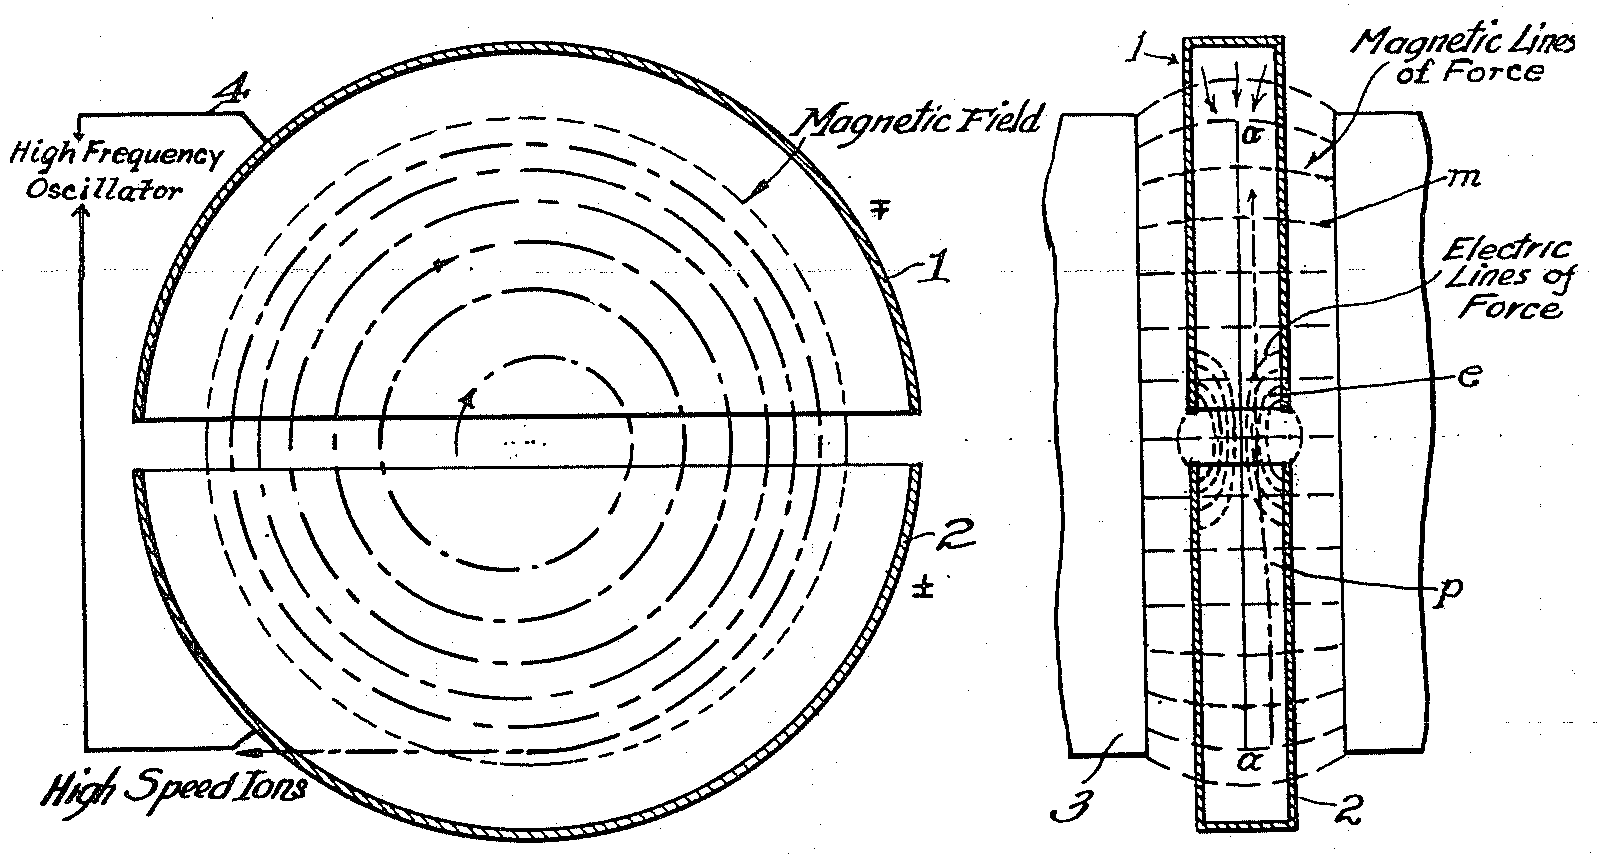
\includegraphics[width=\linewidth]{ Cyclotron_patent.png}
{\color{gray} Ernest O. Lawrence, 1934, U.S. Patent 1,948,384; image in Public Domain.}
\end{column}
\end{columns}
\end{frame}



\begin{frame}
\frametitle{can it be simulated}
\begin{columns}
\begin{column}{0.5\linewidth}
\begin{itemize}
\item<1-> with fixed step size, looks bad 4999 points

\item<2- > my adabtive method, error: $10^{-6}$

\item<2- > Looks great but 2 million points.

\item<3-> odeint library

\item<4-> non-continuous ode are bad.

\end{itemize}
\end{column}
\begin{column}{0.5\linewidth}
\only<1>{%
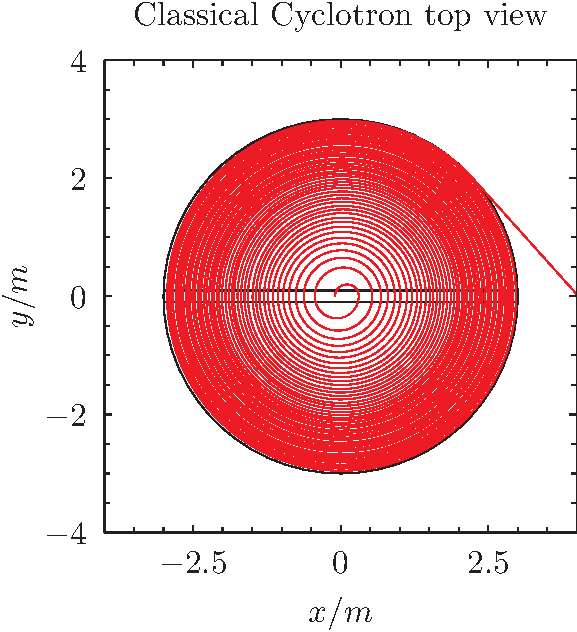
\includegraphics[width=\linewidth]{ cyclotron_noadapt_xy-view.pdf}%

}%
\only<2>{%
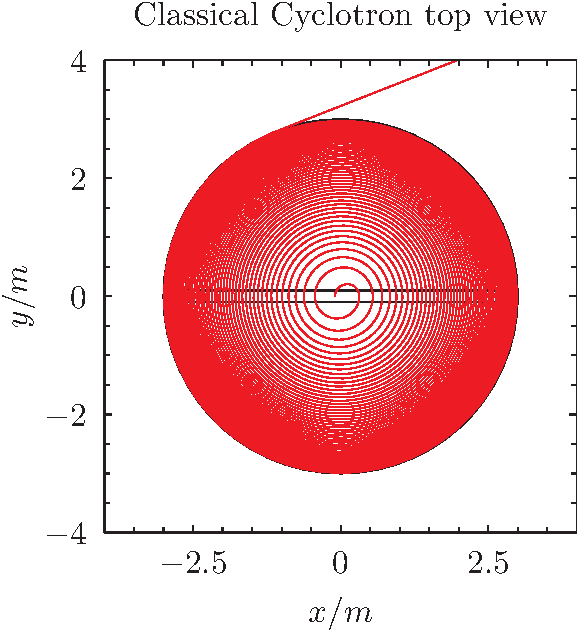
\includegraphics[width=\linewidth]{ cyclotron_overadapt_xy-view.pdf}%

}%
\only<3->{%
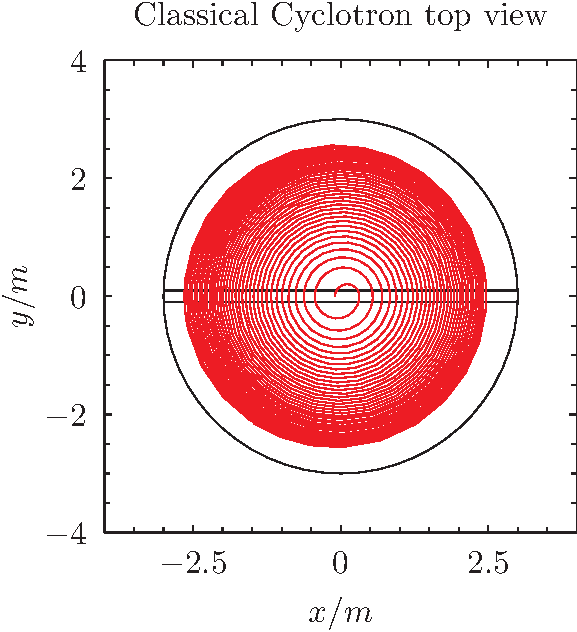
\includegraphics[width=\linewidth]{ cyclotron_badadapt_xy-view.pdf}%
}%

\end{column}
\end{columns}
\end{frame}


%\subsection{If time permits, Cycloid motion.}
%\subsection{If time permits, Toroidal coils.}

\end{document}
